%!TEX program = xelatex
\documentclass[10pt]{article}
\usepackage{ctex}
\usepackage[
colorlinks, 
linkcolor=purple, 
pdfauthor=Guanxu (Gleason) WANG
]{hyperref}
%\usepackage{ctex}
\usepackage{geometry, fancyhdr}
\geometry{
	a4paper,
%	margin=1.6cm,
	left=1cm,
	right=1cm,
	bottom=1.3cm,
	top=2cm,
	headheight=0.5cm,
	footskip=0.3cm}
\linespread{1.1}
\usepackage[leqno]{amsmath}
\usepackage{mathtools, amssymb, mathrsfs, bbm, extpfeil, enumitem}
\usepackage{wrapfig, graphicx, subcaption, multirow, multicol, longtable, booktabs, makecell, pdflscape}
\usepackage{tikz, pgfplots}
\usetikzlibrary{patterns,arrows.meta,calc}
\everymath{\displaystyle}

\pagestyle{fancy}
\renewcommand{\headrulewidth}{0pt}
\fancyhf{}
\fancyhead[R]{\includegraphics[height=1cm]{Lumist.png}}
\fancyfoot[C]{\thepage}

\tolerance=1
\emergencystretch=\maxdimen
\hyphenpenalty=10000
\hbadness=10000

\definecolor{Lumist}{HTML}{F6CA5E}

\usepackage{tocloft}
\renewcommand{\contentsname}{}

\usepackage{eso-pic}
\AddToShipoutPictureBG{
	\begin{tikzpicture}[remember picture, overlay]
		\foreach \x in {0, 10, 20}
		{
			\foreach \y in {-40, -30, ..., 40}
			{
				\node[
				opacity=0.2,
				scale=0.8
				] at (\x,\y)
				{\includegraphics[height=1cm]{Lumist.png}};
			}
		}
		\foreach \x in {5, 15}
		{
			\foreach \y in {-45, -35, ..., 45}
			{
				\node[
				opacity=0.2,
				scale=0.8
				] at (\x,\y)
				{\includegraphics[height=1cm]{Lumist.png}};
			}
		}
	\end{tikzpicture}
}


\begin{document}
	
	%%% 封面页
	
	\begin{titlepage}
		\thispagestyle{empty}
		\tikz[overlay]\path[opacity=0.2](0,0); 
		\begin{tikzpicture}[remember picture, overlay]
			
			% 顶部颜色条
			\fill[Lumist]
			(current page.north west)
			rectangle ([yshift=-6cm]current page.north east);
			
			\node[anchor=north west]
			at ([xshift=1.2cm, yshift=-0.6cm]current page.north west)
			{\includegraphics[height=5cm]{LumistMS.png}};
		\end{tikzpicture}
		\centering
		~\par
		\vspace{6.5cm}
		\textsc{\fontsize{35pt}{1}\selectfont Statistical Tables}\par
		\vspace{1cm}
		{\Huge\bfseries 统\quad 计\quad 分\quad 布\quad 表}\par
		\vspace{2cm}
		\vfill
		\textsc{\LARGE 数学与统计学学科组制}\par 
		\vspace{0.5cm}
		{\large \tableofcontents}
		\vspace{2cm}
	\end{titlepage}

	
	%%% 从这里开始编辑内容 %%%
	%%%%%%%%%%%%%%%%%%%%%%%%
	\pagenumbering{arabic}
	\setcounter{page}{1}
	\input{1. Normal distribution}
	\newpage
	\section{Student's $t$ distribution}
\noindent
\begin{minipage}{0.67\textwidth}
	The table below contains the quantiles of Student's $t$ distribution with $\nu$ degrees of freedom.
	For $0<p<1$ the quantile is the value of $x$ for which
	\[
	\Pr(X \le x)=p,
	\qquad \text{where } X\sim t(\nu).
	\]
	Thus
	\[
	x=F_\nu^{-1}(p).
	\]
	
	The table only contains the quantiles for $p\ge \frac12$.
	For $p<\frac12$ quantiles can be obtained by exploiting the symmetry of the $t$ distribution:
	\[
	F_\nu^{-1}(p)=-F_\nu^{-1}(1-p).
	\]
\end{minipage}
\hfill
\begin{minipage}{0.32\textwidth}
	\centering
	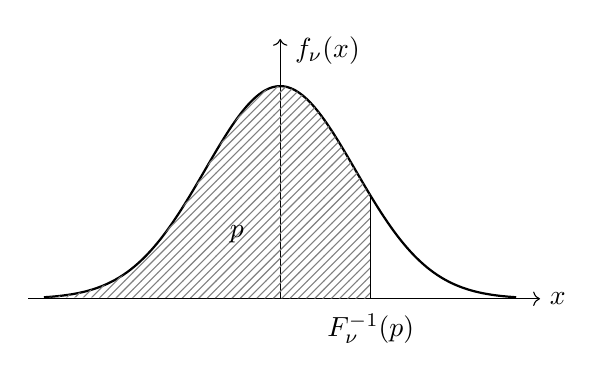
\begin{tikzpicture}[x=1cm, y=1.5cm]
		\draw[->] (-3.2,0) -- (3.3,0) node[right] {$x$};
		\draw[->] (0,0) -- (0,2.2);
		
		\draw[thick,domain=-3:3,smooth,samples=200]
		plot (\x,{1.8*exp(-0.55*\x*\x)});
		
		\fill[pattern=north east lines, pattern color=gray]
		(-3,0)
		plot[domain=-3:1.15,smooth,samples=200]
		(\x,{1.8*exp(-0.55*\x*\x)})
		-- (1.15,0) -- cycle;
		
		\draw[thin] (1.15,0) -- (1.15,{1.8*exp(-0.55*1.15*1.15)});
		
		\node at (-0.55,0.55) {$p$};
		\node[above] at (0.6,1.9) {$f_\nu(x)$};
		\node[below] at (1.15,-0.05) {$F_\nu^{-1}(p)$};
	\end{tikzpicture}
\end{minipage}

\begin{table}[htbp]
	\centering
	%		\caption{}
	%			\scriptsize
	\setlength{\tabcolsep}{7pt}
	%			\renewcommand{\arraystretch}{0.85}
	\begin{tabular}{ccccccccccccc}
		& \multicolumn{12}{c}{$p$}\\
		\cline{2-13}
		df ($\nu$) & 0.6 & 0.7 & 0.75 & 0.8 & 0.85 & 0.9 & 0.95 & 0.975 & 0.99 & 0.995 & 0.999 & 0.9995 \\
		\hline
		1 & 0.3249 & 0.7265 & 1.0000 & 1.3764 & 1.9626 & 3.0777 & 6.3138 & 12.706 & 31.821 & 63.657 & 318.31 & 636.62 \\
		2 & 0.2887 & 0.6172 & 0.8165 & 1.0607 & 1.3862 & 1.8856 & 2.9200 & 4.3027 & 6.9646 & 9.9248 & 22.327 & 31.599 \\
		3 & 0.2767 & 0.5844 & 0.7649 & 0.9785 & 1.2498 & 1.6377 & 2.3534 & 3.1824 & 4.5407 & 5.8409 & 10.215 & 12.924 \\
		4 & 0.2707 & 0.5686 & 0.7407 & 0.9410 & 1.1896 & 1.5332 & 2.1318 & 2.7764 & 3.7469 & 4.6041 & 7.1732 & 8.6103 \\
		5 & 0.2672 & 0.5594 & 0.7267 & 0.9195 & 1.1558 & 1.4759 & 2.0150 & 2.5706 & 3.3649 & 4.0321 & 5.8934 & 6.8688 \\
		6 & 0.2648 & 0.5534 & 0.7176 & 0.9057 & 1.1342 & 1.4398 & 1.9432 & 2.4469 & 3.1427 & 3.7074 & 5.2076 & 5.9588 \\
		7 & 0.2632 & 0.5491 & 0.7111 & 0.8960 & 1.1192 & 1.4149 & 1.8946 & 2.3646 & 2.9980 & 3.4995 & 4.7853 & 5.4079 \\
		8 & 0.2619 & 0.5459 & 0.7064 & 0.8889 & 1.1081 & 1.3968 & 1.8595 & 2.3060 & 2.8965 & 3.3554 & 4.5008 & 5.0413 \\
		9 & 0.2610 & 0.5435 & 0.7027 & 0.8834 & 1.0997 & 1.3830 & 1.8331 & 2.2622 & 2.8214 & 3.2498 & 4.2968 & 4.7809 \\[5pt]
		10 & 0.2602 & 0.5415 & 0.6998 & 0.8791 & 1.0931 & 1.3722 & 1.8125 & 2.2281 & 2.7638 & 3.1693 & 4.1437 & 4.5869 \\
		11 & 0.2596 & 0.5399 & 0.6974 & 0.8755 & 1.0877 & 1.3634 & 1.7959 & 2.2010 & 2.7181 & 3.1058 & 4.0247 & 4.4370 \\
		12 & 0.2590 & 0.5386 & 0.6955 & 0.8726 & 1.0832 & 1.3562 & 1.7823 & 2.1788 & 2.6810 & 3.0545 & 3.9296 & 4.3178 \\
		13 & 0.2586 & 0.5375 & 0.6938 & 0.8702 & 1.0795 & 1.3502 & 1.7709 & 2.1604 & 2.6503 & 3.0123 & 3.8520 & 4.2208 \\
		14 & 0.2582 & 0.5366 & 0.6924 & 0.8681 & 1.0763 & 1.3450 & 1.7613 & 2.1448 & 2.6245 & 2.9768 & 3.7874 & 4.1405 \\
		15 & 0.2579 & 0.5357 & 0.6912 & 0.8662 & 1.0735 & 1.3406 & 1.7531 & 2.1314 & 2.6025 & 2.9467 & 3.7328 & 4.0728 \\
		16 & 0.2576 & 0.5350 & 0.6901 & 0.8647 & 1.0711 & 1.3368 & 1.7459 & 2.1199 & 2.5835 & 2.9208 & 3.6862 & 4.0150 \\
		17 & 0.2573 & 0.5344 & 0.6892 & 0.8633 & 1.0690 & 1.3334 & 1.7396 & 2.1098 & 2.5669 & 2.8982 & 3.6458 & 3.9651 \\
		18 & 0.2571 & 0.5338 & 0.6884 & 0.8620 & 1.0672 & 1.3304 & 1.7341 & 2.1009 & 2.5524 & 2.8784 & 3.6105 & 3.9216 \\
		19 & 0.2569 & 0.5333 & 0.6876 & 0.8610 & 1.0655 & 1.3277 & 1.7291 & 2.0930 & 2.5395 & 2.8609 & 3.5794 & 3.8834 \\[5pt]
		20 & 0.2567 & 0.5329 & 0.6870 & 0.8600 & 1.0640 & 1.3253 & 1.7247 & 2.0860 & 2.5280 & 2.8453 & 3.5518 & 3.8495 \\
		21 & 0.2566 & 0.5325 & 0.6864 & 0.8591 & 1.0627 & 1.3232 & 1.7207 & 2.0796 & 2.5176 & 2.8314 & 3.5272 & 3.8193 \\
		22 & 0.2564 & 0.5321 & 0.6858 & 0.8583 & 1.0614 & 1.3212 & 1.7171 & 2.0739 & 2.5083 & 2.8188 & 3.5050 & 3.7921 \\
		23 & 0.2563 & 0.5317 & 0.6853 & 0.8575 & 1.0603 & 1.3195 & 1.7139 & 2.0687 & 2.4999 & 2.8073 & 3.4850 & 3.7676 \\
		24 & 0.2562 & 0.5314 & 0.6848 & 0.8569 & 1.0593 & 1.3178 & 1.7109 & 2.0639 & 2.4922 & 2.7969 & 3.4668 & 3.7454 \\
		25 & 0.2561 & 0.5312 & 0.6844 & 0.8562 & 1.0584 & 1.3163 & 1.7081 & 2.0595 & 2.4851 & 2.7874 & 3.4502 & 3.7251 \\
		26 & 0.2560 & 0.5309 & 0.6840 & 0.8557 & 1.0575 & 1.3150 & 1.7056 & 2.0555 & 2.4786 & 2.7787 & 3.4350 & 3.7066 \\
		27 & 0.2559 & 0.5306 & 0.6837 & 0.8551 & 1.0567 & 1.3137 & 1.7033 & 2.0518 & 2.4727 & 2.7707 & 3.4210 & 3.6896 \\
		28 & 0.2558 & 0.5304 & 0.6834 & 0.8546 & 1.0560 & 1.3125 & 1.7011 & 2.0484 & 2.4671 & 2.7633 & 3.4082 & 3.6739 \\
		29 & 0.2557 & 0.5302 & 0.6830 & 0.8542 & 1.0553 & 1.3114 & 1.6991 & 2.0452 & 2.4620 & 2.7564 & 3.3962 & 3.6594 \\[5pt]
		30 & 0.2556 & 0.5300 & 0.6828 & 0.8538 & 1.0547 & 1.3104 & 1.6973 & 2.0423 & 2.4573 & 2.7500 & 3.3852 & 3.6460 \\
		40 & 0.2550 & 0.5286 & 0.6807 & 0.8507 & 1.0500 & 1.3031 & 1.6839 & 2.0211 & 2.4233 & 2.7045 & 3.3069 & 3.5510 \\
		50 & 0.2547 & 0.5278 & 0.6794 & 0.8489 & 1.0473 & 1.2987 & 1.6759 & 2.0086 & 2.4033 & 2.6778 & 3.2614 & 3.4960 \\
		60 & 0.2545 & 0.5272 & 0.6786 & 0.8477 & 1.0455 & 1.2958 & 1.6706 & 2.0003 & 2.3901 & 2.6603 & 3.2317 & 3.4602 \\
		80 & 0.2542 & 0.5265 & 0.6776 & 0.8461 & 1.0432 & 1.2922 & 1.6641 & 1.9901 & 2.3739 & 2.6387 & 3.1953 & 3.4163 \\
		100 & 0.2540 & 0.5261 & 0.6770 & 0.8452 & 1.0418 & 1.2901 & 1.6602 & 1.9840 & 2.3642 & 2.6259 & 3.1737 & 3.3905 \\
		120 & 0.2539 & 0.5258 & 0.6765 & 0.8446 & 1.0409 & 1.2886 & 1.6577 & 1.9799 & 2.3578 & 2.6174 & 3.1595 & 3.3735 \\
		150 & 0.2538 & 0.5255 & 0.6761 & 0.8440 & 1.0400 & 1.2872 & 1.6551 & 1.9759 & 2.3515 & 2.6090 & 3.1455 & 3.3566 \\
		200 & 0.2537 & 0.5252 & 0.6757 & 0.8434 & 1.0391 & 1.2858 & 1.6525 & 1.9719 & 2.3451 & 2.6006 & 3.1315 & 3.3398 \\
		500 & 0.2535 & 0.5247 & 0.6750 & 0.8423 & 1.0375 & 1.2832 & 1.6479 & 1.9647 & 2.3338 & 2.5857 & 3.1066 & 3.3101 \\
		\hline
	\end{tabular}
\end{table}

	\newpage
	\section{$\chi^2$ distribution}
\noindent
\begin{minipage}{0.67\textwidth}
	The table below contains the quantiles of the \(\chi^2\) (chi-squared) distribution with \(\nu\) degrees of freedom.
	For \(0<p<1\) the quantile is the value of \(x\) for which
	\[
	\Pr(X\le x)=p,
	\qquad \text{where } X\sim \chi^2(\nu).
	\]
	Thus
	\[
	x = F_\nu^{-1}(p).
	\]
\end{minipage}
\hfill
\begin{minipage}{0.32\textwidth}
	\centering
	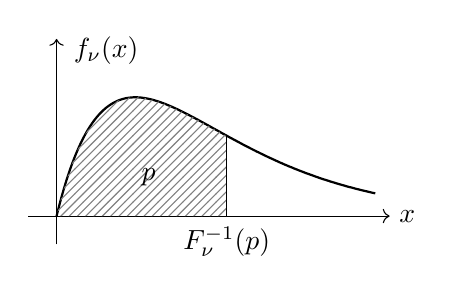
\begin{tikzpicture}[scale=0.9]
		\draw[->] (-0.4,0) -- (4.7,0) node[right] {$x$};
		\draw[->] (0,-0.4) -- (0,2.5);
		
		\draw[thick,domain=0:4.5,smooth,samples=200]
		plot (\x,{4.1*\x*exp(-0.9*\x)});
		
		\fill[pattern=north east lines, pattern color=gray]
		(0,0)
		plot[domain=0:2.4,smooth,samples=200]
		(\x,{4.1*\x*exp(-0.9*\x)})
		-- (2.4,0) -- cycle;
		
		\draw[thin] (2.4,0) -- (2.4,{4.1*2.4*exp(-0.9*2.4)});
		
		\node at (1.3,0.55) {$p$};
		\node[above] at (0.7,2.0) {$f_\nu(x)$};
		\node[below] at (2.4,-0.02) {$F_\nu^{-1}(p)$};
	\end{tikzpicture}
\end{minipage}

\vspace{1em}

\setlength{\LTleft}{0pt}
\setlength{\LTright}{0pt}

\begin{table}[htbp]
	\centering
	%		\caption{}
	%			\scriptsize
	\setlength{\tabcolsep}{7pt}
	%			\renewcommand{\arraystretch}{0.85}
	\begin{tabular}{ccccccccccccc}
		& \multicolumn{12}{c}{$p$}\\
		\cline{2-13}
		df ($\nu$) & 0.005 & 0.01 & 0.025 & 0.05 & 0.1 & 0.5 & 0.9 & 0.95 & 0.975 & 0.99 & 0.995 & 0.999 \\
		\hline
		1   & 0.0000 & 0.0002 & 0.0010 & 0.0039 & 0.0158 & 0.4549 & 2.7055 & 3.8415 & 5.0239 & 6.6349 & 7.8794 & 10.828 \\
		2   & 0.0100 & 0.0201 & 0.0506 & 0.1026 & 0.2107 & 1.3863 & 4.6052 & 5.9915 & 7.3778 & 9.2103 & 10.597 & 13.816 \\
		3   & 0.0717 & 0.1148 & 0.2158 & 0.3518 & 0.5844 & 2.3660 & 6.2514 & 7.8147 & 9.3484 & 11.345 & 12.838 & 16.266 \\
		4   & 0.2070 & 0.2971 & 0.4844 & 0.7107 & 1.0636 & 3.3567 & 7.7794 & 9.4877 & 11.143 & 13.277 & 14.860 & 18.467 \\
		5   & 0.4117 & 0.5543 & 0.8312 & 1.1455 & 1.6103 & 4.3515 & 9.2364 & 11.070 & 12.833 & 15.086 & 16.750 & 20.515 \\
		6   & 0.6757 & 0.8721 & 1.2373 & 1.6354 & 2.2041 & 5.3481 & 10.645 & 12.592 & 14.449 & 16.812 & 18.548 & 22.458 \\
		7   & 0.9893 & 1.2390 & 1.6899 & 2.1673 & 2.8331 & 6.3458 & 12.017 & 14.067 & 16.013 & 18.475 & 20.278 & 24.322 \\
		8   & 1.3444 & 1.6465 & 2.1797 & 2.7326 & 3.4895 & 7.3441 & 13.362 & 15.507 & 17.535 & 20.090 & 21.955 & 26.124 \\
		9   & 1.7349 & 2.0879 & 2.7004 & 3.3251 & 4.1682 & 8.3428 & 14.684 & 16.919 & 19.023 & 21.666 & 23.589 & 27.877 \\[5pt]
		10  & 2.1559 & 2.5582 & 3.2470 & 3.9403 & 4.8652 & 9.3418 & 15.987 & 18.307 & 20.483 & 23.209 & 25.188 & 29.588 \\
		11  & 2.6032 & 3.0535 & 3.8157 & 4.5748 & 5.5778 & 10.341 & 17.275 & 19.675 & 21.920 & 24.725 & 26.757 & 31.264 \\
		12  & 3.0738 & 3.5706 & 4.4038 & 5.2260 & 6.3038 & 11.340 & 18.549 & 21.026 & 23.337 & 26.217 & 28.300 & 32.909 \\
		13  & 3.5650 & 4.1069 & 5.0088 & 5.8919 & 7.0415 & 12.340 & 19.812 & 22.362 & 24.736 & 27.688 & 29.819 & 34.528 \\
		14  & 4.0747 & 4.6604 & 5.6287 & 6.5706 & 7.7895 & 13.339 & 21.064 & 23.685 & 26.119 & 29.141 & 31.319 & 36.123 \\
		15  & 4.6009 & 5.2293 & 6.2621 & 7.2609 & 8.5468 & 14.339 & 22.307 & 24.996 & 27.488 & 30.578 & 32.801 & 37.697 \\
		16  & 5.1422 & 5.8122 & 6.9077 & 7.9616 & 9.3122 & 15.338 & 23.542 & 26.296 & 28.845 & 32.000 & 34.267 & 39.252 \\
		17  & 5.6972 & 6.4078 & 7.5642 & 8.6718 & 10.085 & 16.338 & 24.769 & 27.587 & 30.191 & 33.409 & 35.718 & 40.790 \\
		18  & 6.2648 & 7.0149 & 8.2307 & 9.3905 & 10.865 & 17.338 & 25.989 & 28.869 & 31.526 & 34.805 & 37.156 & 42.312 \\
		19  & 6.8440 & 7.6327 & 8.9065 & 10.117 & 11.651 & 18.338 & 27.204 & 30.144 & 32.852 & 36.191 & 38.582 & 43.820 \\[5pt]
		20  & 7.4338 & 8.2604 & 9.5908 & 10.851 & 12.443 & 19.337 & 28.412 & 31.410 & 34.170 & 37.566 & 39.997 & 45.315 \\
		21  & 8.0337 & 8.8972 & 10.283 & 11.591 & 13.240 & 20.337 & 29.615 & 32.671 & 35.479 & 38.932 & 41.401 & 46.797 \\
		22  & 8.6427 & 9.5425 & 10.982 & 12.338 & 14.041 & 21.337 & 30.813 & 33.924 & 36.781 & 40.289 & 42.796 & 48.268 \\
		23  & 9.2604 & 10.196 & 11.689 & 13.091 & 14.848 & 22.337 & 32.007 & 35.172 & 38.076 & 41.638 & 44.181 & 49.728 \\
		24  & 9.8862 & 10.856 & 12.401 & 13.848 & 15.659 & 23.337 & 33.196 & 36.415 & 39.364 & 42.980 & 45.559 & 51.179 \\
		25  & 10.520 & 11.524 & 13.120 & 14.611 & 16.473 & 24.337 & 34.382 & 37.652 & 40.646 & 44.314 & 46.928 & 52.620 \\
		26  & 11.160 & 12.198 & 13.844 & 15.379 & 17.292 & 25.336 & 35.563 & 38.885 & 41.923 & 45.642 & 48.290 & 54.052 \\
		27  & 11.808 & 12.879 & 14.573 & 16.151 & 18.114 & 26.336 & 36.741 & 40.113 & 43.195 & 46.963 & 49.645 & 55.476 \\
		28  & 12.461 & 13.565 & 15.308 & 16.928 & 18.939 & 27.336 & 37.916 & 41.337 & 44.461 & 48.278 & 50.993 & 56.892 \\
		29  & 13.121 & 14.256 & 16.047 & 17.708 & 19.768 & 28.336 & 39.087 & 42.557 & 45.722 & 49.588 & 52.336 & 58.301 \\[5pt]
		30  & 13.787 & 14.953 & 16.791 & 18.493 & 20.599 & 29.336 & 40.256 & 43.773 & 46.979 & 50.892 & 53.672 & 59.703 \\
		40  & 20.707 & 22.164 & 24.433 & 26.509 & 29.051 & 39.335 & 51.805 & 55.758 & 59.342 & 63.691 & 66.766 & 73.402 \\
		50  & 27.991 & 29.707 & 32.357 & 34.764 & 37.689 & 49.335 & 63.167 & 67.505 & 71.420 & 76.154 & 79.490 & 86.661 \\
		60  & 35.534 & 37.485 & 40.482 & 43.188 & 46.459 & 59.335 & 74.397 & 79.082 & 83.298 & 88.379 & 91.952 & 99.607 \\
		70  & 43.275 & 45.442 & 48.758 & 51.739 & 55.329 & 69.334 & 85.527 & 90.531 & 95.023 & 100.43 & 104.21 & 112.32 \\
		80  & 51.172 & 53.540 & 57.153 & 60.391 & 64.278 & 79.334 & 96.578 & 101.88 & 106.63 & 112.33 & 116.32 & 124.84 \\
		90  & 59.196 & 61.754 & 65.647 & 69.126 & 73.291 & 89.334 & 107.57 & 113.15 & 118.14 & 124.12 & 128.30 & 137.21 \\[5pt]
		100 & 67.328 & 70.065 & 74.222 & 77.929 & 82.358 & 99.334 & 118.50 & 124.34 & 129.56 & 135.81 & 140.17 & 149.45 \\
		120 & 83.852 & 86.923 & 91.573 & 95.705 & 100.62 & 119.33 & 140.23 & 146.57 & 152.21 & 158.95 & 163.65 & 173.62 \\
		150 & 109.14 & 112.67 & 117.98 & 122.69 & 128.28 & 149.33 & 172.58 & 179.58 & 185.80 & 193.21 & 198.36 & 209.26 \\
		200 & 152.24 & 156.43 & 162.73 & 168.28 & 174.84 & 199.33 & 226.02 & 233.99 & 241.06 & 249.45 & 255.26 & 267.54 \\
		500 & 422.30 & 429.39 & 439.94 & 449.15 & 459.93 & 499.33 & 540.93 & 553.13 & 563.85 & 576.49 & 585.21 & 603.45 \\
		\hline
	\end{tabular}
\end{table}
	\newpage
	\section{$F$ distribution}
\noindent
\begin{minipage}{0.67\textwidth}
	The table below contains the quantiles of the F distribution with
	$\nu_1$ and $\nu_2$ degrees of freedom.
	For 0<p<1, the quantile is the value of x for which
	\[
	\Pr\{X\le x\}=p,
	\qquad
	\text{where } X\sim F(\nu_1,\nu_2).
	\]
	
	Thus
	\[
	x=F^{-1}_{(\nu_1,\nu_2)}(p).
	\]
	
	The table only contains the quantiles for $p\ge \frac12$.
	For $p<\frac12$, quantiles can be obtained by exploiting the
	symmetry of the F distribution:
	\[
	F^{-1}_{(\nu_1,\nu_2)}(p)
	=
	\frac{1}{
		F^{-1}_{(\nu_2,\nu_1)}(1-p)
	}.
	\]
\end{minipage}
\hfill
\begin{minipage}{0.32\textwidth}
	\centering
	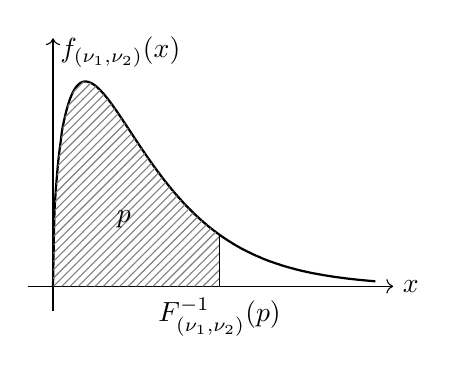
\begin{tikzpicture}[scale=0.9]
		% axes
		\draw[->] (-0.35,0) -- (4.8,0) node[right] {$x$};
		\draw[->] (0,-0.35) -- (0,3.5);
		
		% F-like density curve
		\draw[thick,domain=0.:4.55,smooth,samples=250]
		plot (\x,{3*(\x^0.35+1.7*\x^.75)*exp(-1.25*\x)});
		
		% shaded probability area
		\fill[pattern=north east lines, pattern color=gray]
		(0,0)
		-- plot[domain=0:2.35,smooth,samples=200]
		(\x,{3*(\x^0.35+1.7*\x^.75)*exp(-1.25*\x)})
		-- (2.35,0)
		-- cycle;
		
		% vertical quantile line
		\draw[thin] 
		(2.35,0) -- (2.35,{3*(2.35^0.35+1.7*2.35^.75)*exp(-1.25*2.35)});
		
		% labels
		\node at (1,0.95) {$p$};
		\node[above] at (0.95,2.95) {$f_{(\nu_1,\nu_2)}(x)$};
		\node[below] at (2.35,-0.02) {$F^{-1}_{(\nu_1,\nu_2)}(p)$};
	\end{tikzpicture}
\end{minipage}

~\\

\noindent
\begin{minipage}{0.49\textwidth}
	\begin{center}
		\begin{tabular}{ccccccc}
			& & \multicolumn{5}{c}{$p$}\\
			\cline{3-7}
			$\nu_1$ & $\nu_2$ & 0.9 & 0.95 & 0.975 & 0.99 & 0.995 \\
			\midrule
			1 & 1 & 39.863 & 161.45 & 647.79 & 4052.2 & 16211 \\
			& 2 & 8.5263 & 18.513 & 38.506 & 98.503 & 198.50 \\
			& 3 & 5.5383 & 10.128 & 17.443 & 34.116 & 55.552 \\
			& 4 & 4.5448 & 7.7086 & 12.218 & 21.198 & 31.333 \\
			& 5 & 4.0604 & 6.6079 & 10.007 & 16.258 & 22.785 \\
			& 6 & 3.7759 & 5.9874 & 8.8131 & 13.745 & 18.635 \\
			& 7 & 3.5894 & 5.5914 & 8.0727 & 12.246 & 16.236 \\
			& 8 & 3.4579 & 5.3177 & 7.5709 & 11.259 & 14.688 \\
			& 9 & 3.3603 & 5.1174 & 7.2093 & 10.561 & 13.614 \\[5pt]
			& 10 & 3.2850 & 4.9646 & 6.9367 & 10.044 & 12.826 \\
			& 11 & 3.2252 & 4.8443 & 6.7241 & 9.6460 & 12.226 \\
			& 12 & 3.1765 & 4.7472 & 6.5538 & 9.3302 & 11.754 \\
			& 13 & 3.1362 & 4.6672 & 6.4143 & 9.0738 & 11.374 \\
			& 14 & 3.1022 & 4.6001 & 6.2979 & 8.8616 & 11.060 \\
			& 15 & 3.0732 & 4.5431 & 6.1995 & 8.6831 & 10.798 \\
			& 16 & 3.0481 & 4.4940 & 6.1151 & 8.5310 & 10.575 \\
			& 17 & 3.0262 & 4.4513 & 6.0420 & 8.3997 & 10.384 \\
			& 18 & 3.0070 & 4.4139 & 5.9781 & 8.2854 & 10.218 \\
			& 19 & 2.9899 & 4.3807 & 5.9216 & 8.1849 & 10.073 \\[5pt]
			& 20 & 2.9747 & 4.3512 & 5.8715 & 8.0960 & 9.9439 \\
			& 21 & 2.9610 & 4.3248 & 5.8266 & 8.0166 & 9.8295 \\
			& 22 & 2.9486 & 4.3009 & 5.7863 & 7.9454 & 9.7271 \\
			& 23 & 2.9374 & 4.2793 & 5.7498 & 7.8811 & 9.6348 \\
			& 24 & 2.9271 & 4.2597 & 5.7166 & 7.8229 & 9.5513 \\
			& 25 & 2.9177 & 4.2417 & 5.6864 & 7.7698 & 9.4753 \\
			& 30 & 2.8807 & 4.1709 & 5.5675 & 7.5625 & 9.1797 \\
			& 35 & 2.8547 & 4.1213 & 5.4848 & 7.4191 & 8.9763 \\
			& 40 & 2.8354 & 4.0847 & 5.4239 & 7.3141 & 8.8279 \\
			& 45 & 2.8205 & 4.0566 & 5.3773 & 7.2339 & 8.7148 \\[5pt]
			& 50 & 2.8087 & 4.0343 & 5.3403 & 7.1706 & 8.6258 \\
			& 60 & 2.7911 & 4.0012 & 5.2856 & 7.0771 & 8.4946 \\
			& 70 & 2.7786 & 3.9778 & 5.2470 & 7.0114 & 8.4027 \\
			& 80 & 2.7693 & 3.9604 & 5.2184 & 6.9627 & 8.3346 \\
			& 100 & 2.7564 & 3.9361 & 5.1786 & 6.8953 & 8.2406 \\
			& 120 & 2.7478 & 3.9201 & 5.1523 & 6.8509 & 8.1788 \\
			& 150 & 2.7393 & 3.9042 & 5.1263 & 6.8069 & 8.1177 \\
			& 200 & 2.7308 & 3.8884 & 5.1004 & 6.7633 & 8.0572 \\
			&  &  &  &  &  & $\rightarrow$ \\
		\end{tabular}
	\end{center}
\end{minipage}
\hfill
\begin{minipage}{0.49\textwidth}
	\begin{center}
		\begin{tabular}{ccccccc}
			& & \multicolumn{5}{c}{$p$}\\
			\cline{3-7}
			$\nu_1$ & $\nu_2$ & 0.9 & 0.95 & 0.975 & 0.99 & 0.995 \\
			\midrule
			1 & 500 & 2.7156 & 3.8601 & 5.0543 & 6.6858 & 7.9498 \\
			& $+\infty$ & 2.7055 & 3.8415 & 5.0239 & 6.6349 & 7.8794 \\
			\midrule
			2 & 1 & 49.500 & 199.50 & 799.50 & 4999.5 & 19999 \\
			& 2 & 9.0000 & 19.000 & 39.000 & 99.000 & 199.00 \\
			& 3 & 5.4624 & 9.5521 & 16.044 & 30.817 & 49.799 \\
			& 4 & 4.3246 & 6.9443 & 10.649 & 18.000 & 26.284 \\
			& 5 & 3.7797 & 5.7861 & 8.4336 & 13.274 & 18.314 \\
			& 6 & 3.4633 & 5.1433 & 7.2599 & 10.925 & 14.544 \\
			& 7 & 3.2574 & 4.7374 & 6.5415 & 9.5466 & 12.404 \\
			& 8 & 3.1131 & 4.4590 & 6.0595 & 8.6491 & 11.042 \\
			& 9 & 3.0065 & 4.2565 & 5.7147 & 8.0215 & 10.107 \\[5pt]
			& 10 & 2.9245 & 4.1028 & 5.4564 & 7.5594 & 9.4270 \\
			& 11 & 2.8595 & 3.9823 & 5.2559 & 7.2057 & 8.9122 \\
			& 12 & 2.8068 & 3.8853 & 5.0959 & 6.9266 & 8.5096 \\
			& 13 & 2.7632 & 3.8056 & 4.9653 & 6.7010 & 8.1865 \\
			& 14 & 2.7265 & 3.7389 & 4.8567 & 6.5149 & 7.9216 \\
			& 15 & 2.6952 & 3.6823 & 4.7650 & 6.3589 & 7.7008 \\
			& 16 & 2.6682 & 3.6337 & 4.6867 & 6.2262 & 7.5138 \\
			& 17 & 2.6446 & 3.5915 & 4.6189 & 6.1121 & 7.3536 \\
			& 18 & 2.6239 & 3.5546 & 4.5597 & 6.0129 & 7.2148 \\
			& 19 & 2.6056 & 3.5219 & 4.5075 & 5.9259 & 7.0935 \\[5pt]
			& 20 & 2.5893 & 3.4928 & 4.4613 & 5.8489 & 6.9865 \\
			& 21 & 2.5746 & 3.4668 & 4.4199 & 5.7804 & 6.8914 \\
			& 22 & 2.5613 & 3.4434 & 4.3828 & 5.7190 & 6.8064 \\
			& 23 & 2.5493 & 3.4221 & 4.3492 & 5.6637 & 6.7300 \\
			& 24 & 2.5383 & 3.4028 & 4.3187 & 5.6136 & 6.6609 \\
			& 25 & 2.5283 & 3.3852 & 4.2909 & 5.5680 & 6.5982 \\
			& 30 & 2.4887 & 3.3158 & 4.1821 & 5.3903 & 6.3547 \\
			& 35 & 2.4609 & 3.2674 & 4.1065 & 5.2679 & 6.1878 \\
			& 40 & 2.4404 & 3.2317 & 4.0510 & 5.1785 & 6.0664 \\
			& 45 & 2.4245 & 3.2043 & 4.0085 & 5.1103 & 5.9741 \\[5pt]
			& 50 & 2.4120 & 3.1826 & 3.9749 & 5.0566 & 5.9016 \\
			& 60 & 2.3933 & 3.1504 & 3.9253 & 4.9774 & 5.7950 \\
			& 70 & 2.3800 & 3.1277 & 3.8903 & 4.9219 & 5.7204 \\
			& 80 & 2.3701 & 3.1108 & 3.8643 & 4.8807 & 5.6652 \\
			& 100 & 2.3564 & 3.0873 & 3.8284 & 4.8239 & 5.5892 \\
			& 120 & 2.3473 & 3.0718 & 3.8046 & 4.7865 & 5.5393 \\
			&  &  &  &  &  & $\rightarrow$ \\
		\end{tabular}
	\end{center}
\end{minipage}

\newpage
\noindent
\begin{minipage}{0.49\textwidth}
	\begin{center}
		\begin{tabular}{ccccccc}
			& & \multicolumn{5}{c}{$p$}\\
			\cline{3-7}
			$\nu_1$ & $\nu_2$ & 0.9 & 0.95 & 0.975 & 0.99 & 0.995 \\
			\midrule
			2 & 150 & 2.3383 & 3.0564 & 3.7811 & 4.7495 & 5.4900 \\
			& 200 & 2.3293 & 3.0411 & 3.7578 & 4.7129 & 5.4412 \\
			& 500 & 2.3132 & 3.0138 & 3.7162 & 4.6478 & 5.3549 \\
			& $+\infty$ & 2.3026 & 2.9957 & 3.6889 & 4.6052 & 5.2983 \\
			\midrule
			3 & 1 & 53.593 & 215.71 & 864.16 & 5403.4 & 21615 \\
			& 2 & 9.1618 & 19.164 & 39.165 & 99.166 & 199.17 \\
			& 3 & 5.3908 & 9.2766 & 15.439 & 29.457 & 47.467 \\
			& 4 & 4.1909 & 6.5914 & 9.9792 & 16.694 & 24.259 \\
			& 5 & 3.6195 & 5.4095 & 7.7636 & 12.060 & 16.530 \\
			& 6 & 3.2888 & 4.7571 & 6.5988 & 9.7795 & 12.917 \\
			& 7 & 3.0741 & 4.3468 & 5.8898 & 8.4513 & 10.882 \\
			& 8 & 2.9238 & 4.0662 & 5.4160 & 7.5910 & 9.5965 \\
			& 9 & 2.8129 & 3.8625 & 5.0781 & 6.9919 & 8.7171 \\[5pt]
			& 10 & 2.7277 & 3.7083 & 4.8256 & 6.5523 & 8.0807 \\
			& 11 & 2.6602 & 3.5874 & 4.6300 & 6.2167 & 7.6004 \\
			& 12 & 2.6055 & 3.4903 & 4.4742 & 5.9525 & 7.2258 \\
			& 13 & 2.5603 & 3.4105 & 4.3472 & 5.7394 & 6.9258 \\
			& 14 & 2.5222 & 3.3439 & 4.2417 & 5.5639 & 6.6804 \\
			& 15 & 2.4898 & 3.2874 & 4.1528 & 5.4170 & 6.4760 \\
			& 16 & 2.4618 & 3.2389 & 4.0768 & 5.2922 & 6.3034 \\
			& 17 & 2.4374 & 3.1968 & 4.0112 & 5.1850 & 6.1556 \\
			& 18 & 2.4160 & 3.1599 & 3.9539 & 5.0919 & 6.0278 \\
			& 19 & 2.3970 & 3.1274 & 3.9034 & 5.0103 & 5.9161 \\[5pt]
			& 20 & 2.3801 & 3.0984 & 3.8587 & 4.9382 & 5.8177 \\
			& 21 & 2.3649 & 3.0725 & 3.8188 & 4.8740 & 5.7304 \\
			& 22 & 2.3512 & 3.0491 & 3.7829 & 4.8166 & 5.6524 \\
			& 23 & 2.3387 & 3.0280 & 3.7505 & 4.7649 & 5.5823 \\
			& 24 & 2.3274 & 3.0088 & 3.7211 & 4.7181 & 5.5190 \\
			& 25 & 2.3170 & 2.9912 & 3.6943 & 4.6755 & 5.4615 \\
			& 30 & 2.2761 & 2.9223 & 3.5894 & 4.5097 & 5.2388 \\
			& 35 & 2.2474 & 2.8742 & 3.5166 & 4.3957 & 5.0865 \\
			& 40 & 2.2261 & 2.8387 & 3.4633 & 4.3126 & 4.9758 \\
			& 45 & 2.2097 & 2.8115 & 3.4224 & 4.2492 & 4.8918 \\[5pt]
			& 50 & 2.1967 & 2.7900 & 3.3902 & 4.1993 & 4.8259 \\
			& 60 & 2.1774 & 2.7581 & 3.3425 & 4.1259 & 4.7290 \\
			& 70 & 2.1637 & 2.7355 & 3.3090 & 4.0744 & 4.6613 \\
			& 80 & 2.1535 & 2.7188 & 3.2841 & 4.0363 & 4.6113 \\
			& 100 & 2.1394 & 2.6955 & 3.2496 & 3.9837 & 4.5424 \\
			& 120 & 2.1300 & 2.6802 & 3.2269 & 3.9491 & 4.4972 \\
			& 150 & 2.1207 & 2.6649 & 3.2044 & 3.9149 & 4.4525 \\
			& 200 & 2.1114 & 2.6498 & 3.1820 & 3.8810 & 4.4084 \\
			& 500 & 2.0948 & 2.6227 & 3.1423 & 3.8210 & 4.3304 \\
			& $+\infty$ & 2.0838 & 2.6049 & 3.1161 & 3.7816 & 4.2794 \\
			\midrule
			4 & 1 & 55.833 & 224.58 & 899.58 & 5624.6 & 22500 \\
			& 2 & 9.2434 & 19.247 & 39.248 & 99.249 & 199.25 \\
			& 3 & 5.3426 & 9.1172 & 15.101 & 28.710 & 46.195 \\
			& 4 & 4.1072 & 6.3882 & 9.6045 & 15.977 & 23.155 \\
			& 5 & 3.5202 & 5.1922 & 7.3879 & 11.392 & 15.556 \\
			& 6 & 3.1808 & 4.5337 & 6.2272 & 9.1483 & 12.028 \\
			& 7 & 2.9605 & 4.1203 & 5.5226 & 7.8466 & 10.050 \\
			& 8 & 2.8064 & 3.8379 & 5.0526 & 7.0061 & 8.8051 \\
			 &  &  &  &  &  & $\rightarrow$ \\
		\end{tabular}
	\end{center}
\end{minipage}
\hfill
\begin{minipage}{0.49\textwidth}
	\begin{center}
		\begin{tabular}{ccccccc}
			& & \multicolumn{5}{c}{$p$}\\
			\cline{3-7}
			$\nu_1$ & $\nu_2$ & 0.9 & 0.95 & 0.975 & 0.99 & 0.995 \\
			\midrule
			4 & 9 & 2.6927 & 3.6331 & 4.7181 & 6.4221 & 7.9559 \\[5pt]
			& 10 & 2.6053 & 3.4780 & 4.4683 & 5.9943 & 7.3428 \\
			& 11 & 2.5362 & 3.3567 & 4.2751 & 5.6683 & 6.8809 \\
			& 12 & 2.4801 & 3.2592 & 4.1212 & 5.4120 & 6.5211 \\
			& 13 & 2.4337 & 3.1791 & 3.9959 & 5.2053 & 6.2335 \\
			& 14 & 2.3947 & 3.1122 & 3.8919 & 5.0354 & 5.9984 \\
			& 15 & 2.3614 & 3.0556 & 3.8043 & 4.8932 & 5.8029 \\
			& 16 & 2.3327 & 3.0069 & 3.7294 & 4.7726 & 5.6378 \\
			& 17 & 2.3077 & 2.9647 & 3.6648 & 4.6690 & 5.4967 \\
			& 18 & 2.2858 & 2.9277 & 3.6083 & 4.5790 & 5.3746 \\
			& 19 & 2.2663 & 2.8951 & 3.5587 & 4.5003 & 5.2681 \\[5pt]
			& 20 & 2.2489 & 2.8661 & 3.5147 & 4.4307 & 5.1743 \\
			& 21 & 2.2333 & 2.8401 & 3.4754 & 4.3688 & 5.0911 \\
			& 22 & 2.2193 & 2.8167 & 3.4401 & 4.3134 & 5.0168 \\
			& 23 & 2.2065 & 2.7955 & 3.4083 & 4.2636 & 4.9500 \\
			& 24 & 2.1949 & 2.7763 & 3.3794 & 4.2184 & 4.8898 \\
			& 25 & 2.1842 & 2.7587 & 3.3530 & 4.1774 & 4.8351 \\
			& 30 & 2.1422 & 2.6896 & 3.2499 & 4.0179 & 4.6234 \\
			& 35 & 2.1128 & 2.6415 & 3.1785 & 3.9082 & 4.4788 \\
			& 40 & 2.0909 & 2.6060 & 3.1261 & 3.8283 & 4.3738 \\
			& 45 & 2.0742 & 2.5787 & 3.0860 & 3.7674 & 4.2941 \\[5pt]
			& 50 & 2.0608 & 2.5572 & 3.0544 & 3.7195 & 4.2316 \\
			& 60 & 2.0410 & 2.5252 & 3.0077 & 3.6490 & 4.1399 \\
			& 70 & 2.0269 & 2.5027 & 2.9748 & 3.5996 & 4.0758 \\
			& 80 & 2.0165 & 2.4859 & 2.9504 & 3.5631 & 4.0285 \\
			& 100 & 2.0019 & 2.4626 & 2.9166 & 3.5127 & 3.9634 \\
			& 120 & 1.9923 & 2.4472 & 2.8943 & 3.4795 & 3.9207 \\
			& 150 & 1.9827 & 2.4320 & 2.8722 & 3.4467 & 3.8785 \\
			& 200 & 1.9732 & 2.4168 & 2.8503 & 3.4143 & 3.8368 \\
			& 500 & 1.9561 & 2.3898 & 2.8114 & 3.3569 & 3.7632 \\
			& $+\infty$ & 1.9449 & 2.3719 & 2.7858 & 3.3192 & 3.7151 \\
			\midrule
			5 & 1 & 57.240 & 230.16 & 921.85 & 5763.6 & 23056 \\
			& 2 & 9.2926 & 19.296 & 39.298 & 99.299 & 199.30 \\
			& 3 & 5.3092 & 9.0135 & 14.885 & 28.237 & 45.392 \\
			& 4 & 4.0506 & 6.2561 & 9.3645 & 15.522 & 22.456 \\
			& 5 & 3.4530 & 5.0503 & 7.1464 & 10.967 & 14.940 \\
			& 6 & 3.1075 & 4.3874 & 5.9876 & 8.7459 & 11.464 \\
			& 7 & 2.8833 & 3.9715 & 5.2852 & 7.4604 & 9.5221 \\
			& 8 & 2.7264 & 3.6875 & 4.8173 & 6.6318 & 8.3018 \\
			& 9 & 2.6106 & 3.4817 & 4.4844 & 6.0569 & 7.4712 \\[5pt]
			& 10 & 2.5216 & 3.3258 & 4.2361 & 5.6363 & 6.8724 \\
			& 11 & 2.4512 & 3.2039 & 4.0440 & 5.3160 & 6.4217 \\
			& 12 & 2.3940 & 3.1059 & 3.8911 & 5.0643 & 6.0711 \\
			& 13 & 2.3467 & 3.0254 & 3.7667 & 4.8616 & 5.7910 \\
			& 14 & 2.3069 & 2.9582 & 3.6634 & 4.6950 & 5.5623 \\
			& 15 & 2.2730 & 2.9013 & 3.5764 & 4.5556 & 5.3721 \\
			& 16 & 2.2438 & 2.8524 & 3.5021 & 4.4374 & 5.2117 \\
			& 17 & 2.2183 & 2.8100 & 3.4379 & 4.3359 & 5.0746 \\
			& 18 & 2.1958 & 2.7729 & 3.3820 & 4.2479 & 4.9560 \\
			& 19 & 2.1760 & 2.7401 & 3.3327 & 4.1708 & 4.8526 \\
			& 20 & 2.1582 & 2.7109 & 3.2891 & 4.1027 & 4.7616 \\
			&  &  &  &  &  & $\rightarrow$ \\
		\end{tabular}
	\end{center}
\end{minipage}

\newpage
\noindent
\begin{minipage}{0.49\textwidth}
	\begin{center}
		\begin{tabular}{ccccccc}
			& & \multicolumn{5}{c}{$p$}\\
			\cline{3-7}
			$\nu_1$ & $\nu_2$ & 0.9 & 0.95 & 0.975 & 0.99 & 0.995 \\
			\midrule
			5 & 21 & 2.1423 & 2.6848 & 3.2501 & 4.0421 & 4.6809 \\
			& 22 & 2.1279 & 2.6613 & 3.2151 & 3.9880 & 4.6088 \\
			& 23 & 2.1149 & 2.6400 & 3.1835 & 3.9392 & 4.5441 \\
			& 24 & 2.1030 & 2.6207 & 3.1548 & 3.8951 & 4.4857 \\
			& 25 & 2.0922 & 2.6030 & 3.1287 & 3.8550 & 4.4327 \\
			& 30 & 2.0492 & 2.5336 & 3.0265 & 3.6990 & 4.2276 \\
			& 35 & 2.0191 & 2.4851 & 2.9557 & 3.5919 & 4.0876 \\
			& 40 & 1.9968 & 2.4495 & 2.9037 & 3.5138 & 3.9860 \\
			& 45 & 1.9796 & 2.4221 & 2.8640 & 3.4544 & 3.9090 \\[5pt]
			& 50 & 1.9660 & 2.4004 & 2.8327 & 3.4077 & 3.8486 \\
			& 60 & 1.9457 & 2.3683 & 2.7863 & 3.3389 & 3.7599 \\
			& 70 & 1.9313 & 2.3456 & 2.7537 & 3.2907 & 3.6980 \\
			& 80 & 1.9206 & 2.3287 & 2.7295 & 3.2550 & 3.6524 \\
			& 100 & 1.9057 & 2.3053 & 2.6961 & 3.2059 & 3.5895 \\
			& 120 & 1.8959 & 2.2899 & 2.6740 & 3.1735 & 3.5482 \\
			& 150 & 1.8861 & 2.2745 & 2.6521 & 3.1416 & 3.5075 \\
			& 200 & 1.8763 & 2.2592 & 2.6304 & 3.1100 & 3.4674 \\
			& 500 & 1.8588 & 2.2320 & 2.5919 & 3.0540 & 3.3963 \\
			& $+\infty$ & 1.8473 & 2.2141 & 2.5665 & 3.0173 & 3.3499 \\
			\midrule
			6 & 1 & 58.204 & 233.99 & 937.11 & 5859.0 & 23437 \\
			& 2 & 9.3255 & 19.330 & 39.331 & 99.333 & 199.33 \\
			& 3 & 5.2847 & 8.9406 & 14.735 & 27.911 & 44.838 \\
			& 4 & 4.0097 & 6.1631 & 9.1973 & 15.207 & 21.975 \\
			& 5 & 3.4045 & 4.9503 & 6.9777 & 10.672 & 14.513 \\
			& 6 & 3.0546 & 4.2839 & 5.8198 & 8.4661 & 11.073 \\
			& 7 & 2.8274 & 3.8660 & 5.1186 & 7.1914 & 9.1553 \\
			& 8 & 2.6683 & 3.5806 & 4.6517 & 6.3707 & 7.9520 \\
			& 9 & 2.5509 & 3.3738 & 4.3197 & 5.8018 & 7.1339 \\[5pt]
			& 10 & 2.4606 & 3.2172 & 4.0721 & 5.3858 & 6.5446 \\
			& 11 & 2.3891 & 3.0946 & 3.8807 & 5.0692 & 6.1016 \\
			& 12 & 2.3310 & 2.9961 & 3.7283 & 4.8206 & 5.7570 \\
			& 13 & 2.2830 & 2.9153 & 3.6043 & 4.6204 & 5.4819 \\
			& 14 & 2.2426 & 2.8477 & 3.5014 & 4.4558 & 5.2574 \\
			& 15 & 2.2081 & 2.7905 & 3.4147 & 4.3183 & 5.0708 \\
			& 16 & 2.1783 & 2.7413 & 3.3406 & 4.2016 & 4.9134 \\
			& 17 & 2.1524 & 2.6987 & 3.2767 & 4.1015 & 4.7789 \\
			& 18 & 2.1296 & 2.6613 & 3.2209 & 4.0146 & 4.6627 \\
			& 19 & 2.1094 & 2.6283 & 3.1718 & 3.9386 & 4.5614 \\[5pt]
			& 20 & 2.0913 & 2.5990 & 3.1283 & 3.8714 & 4.4721 \\
			& 21 & 2.0751 & 2.5727 & 3.0895 & 3.8117 & 4.3931 \\
			& 22 & 2.0605 & 2.5491 & 3.0546 & 3.7583 & 4.3225 \\
			& 23 & 2.0472 & 2.5277 & 3.0232 & 3.7102 & 4.2591 \\
			& 24 & 2.0351 & 2.5082 & 2.9946 & 3.6667 & 4.2019 \\
			& 25 & 2.0241 & 2.4904 & 2.9685 & 3.6272 & 4.1500 \\
			& 30 & 1.9803 & 2.4205 & 2.8667 & 3.4735 & 3.9492 \\
			& 35 & 1.9496 & 2.3718 & 2.7961 & 3.3679 & 3.8123 \\
			& 40 & 1.9269 & 2.3359 & 2.7444 & 3.2910 & 3.7129 \\
			& 45 & 1.9094 & 2.3083 & 2.7048 & 3.2325 & 3.6376 \\[5pt]
			& 50 & 1.8954 & 2.2864 & 2.6736 & 3.1864 & 3.5785 \\
			& 60 & 1.8747 & 2.2541 & 2.6274 & 3.1187 & 3.4918 \\
			& 70 & 1.8600 & 2.2312 & 2.5949 & 3.0712 & 3.4313 \\
			& 80 & 1.8491 & 2.2142 & 2.5708 & 3.0361 & 3.3867 \\
			&  &  &  &  &  & $\rightarrow$ \\
		\end{tabular}
	\end{center}
\end{minipage}
\hfill
\begin{minipage}{0.49\textwidth}
	\begin{center}
		\begin{tabular}{ccccccc}
			& & \multicolumn{5}{c}{$p$}\\
			\cline{3-7}
			$\nu_1$ & $\nu_2$ & 0.9 & 0.95 & 0.975 & 0.99 & 0.995 \\
			\midrule
			6 & 100 & 1.8339 & 2.1906 & 2.5374 & 2.9877 & 3.3252 \\
			& 120 & 1.8238 & 2.1750 & 2.5154 & 2.9559 & 3.2849 \\
			& 150 & 1.8138 & 2.1595 & 2.4936 & 2.9244 & 3.2452 \\
			& 200 & 1.8038 & 2.1441 & 2.4720 & 2.8933 & 3.2059 \\
			& 500 & 1.7859 & 2.1167 & 2.4335 & 2.8381 & 3.1366 \\
			& $+\infty$ & 1.7741 & 2.0986 & 2.4082 & 2.8020 & 3.0913 \\
			\midrule
			7 & 1 & 58.906 & 236.77 & 948.22 & 5928.4 & 23715 \\
			& 2 & 9.3491 & 19.353 & 39.355 & 99.356 & 199.36 \\
			& 3 & 5.2662 & 8.8867 & 14.624 & 27.672 & 44.434 \\
			& 4 & 3.9790 & 6.0942 & 9.0741 & 14.976 & 21.622 \\
			& 5 & 3.3679 & 4.8759 & 6.8531 & 10.456 & 14.200 \\
			& 6 & 3.0145 & 4.2067 & 5.6955 & 8.2600 & 10.786 \\
			& 7 & 2.7849 & 3.7870 & 4.9949 & 6.9928 & 8.8854 \\
			& 8 & 2.6241 & 3.5005 & 4.5286 & 6.1776 & 7.6941 \\
			& 9 & 2.5053 & 3.2927 & 4.1970 & 5.6129 & 6.8849 \\[5pt]
			& 10 & 2.4140 & 3.1355 & 3.9498 & 5.2001 & 6.3025 \\
			& 11 & 2.3416 & 3.0123 & 3.7586 & 4.8861 & 5.8648 \\
			& 12 & 2.2828 & 2.9134 & 3.6065 & 4.6395 & 5.5245 \\
			& 13 & 2.2341 & 2.8321 & 3.4827 & 4.4410 & 5.2529 \\
			& 14 & 2.1931 & 2.7642 & 3.3799 & 4.2779 & 5.0313 \\
			& 15 & 2.1582 & 2.7066 & 3.2934 & 4.1415 & 4.8473 \\
			& 16 & 2.1280 & 2.6572 & 3.2194 & 4.0259 & 4.6920 \\
			& 17 & 2.1017 & 2.6143 & 3.1556 & 3.9267 & 4.5594 \\
			& 18 & 2.0785 & 2.5767 & 3.0999 & 3.8406 & 4.4448 \\
			& 19 & 2.0580 & 2.5435 & 3.0509 & 3.7653 & 4.3448 \\[5pt]
			& 20 & 2.0397 & 2.5140 & 3.0074 & 3.6987 & 4.2569 \\
			& 21 & 2.0233 & 2.4876 & 2.9686 & 3.6396 & 4.1789 \\
			& 22 & 2.0084 & 2.4638 & 2.9338 & 3.5867 & 4.1094 \\
			& 23 & 1.9949 & 2.4422 & 2.9023 & 3.5390 & 4.0469 \\
			& 24 & 1.9826 & 2.4226 & 2.8738 & 3.4959 & 3.9905 \\
			& 25 & 1.9714 & 2.4047 & 2.8478 & 3.4568 & 3.9394 \\
			& 30 & 1.9269 & 2.3343 & 2.7460 & 3.3045 & 3.7416 \\
			& 35 & 1.8957 & 2.2852 & 2.6755 & 3.2000 & 3.6066 \\
			& 40 & 1.8725 & 2.2490 & 2.6238 & 3.1238 & 3.5088 \\
			& 45 & 1.8547 & 2.2212 & 2.5842 & 3.0658 & 3.4346 \\[5pt]
			& 50 & 1.8405 & 2.1992 & 2.5530 & 3.0202 & 3.3765 \\
			& 60 & 1.8194 & 2.1665 & 2.5068 & 2.9530 & 3.2911 \\
			& 70 & 1.8044 & 2.1435 & 2.4743 & 2.9060 & 3.2315 \\
			& 80 & 1.7933 & 2.1263 & 2.4502 & 2.8713 & 3.1876 \\
			& 100 & 1.7778 & 2.1025 & 2.4168 & 2.8233 & 3.1271 \\
			& 120 & 1.7675 & 2.0868 & 2.3948 & 2.7918 & 3.0874 \\
			& 150 & 1.7572 & 2.0711 & 2.3730 & 2.7606 & 3.0483 \\
			& 200 & 1.7470 & 2.0556 & 2.3513 & 2.7298 & 3.0097 \\
			& 500 & 1.7288 & 2.0279 & 2.3129 & 2.6751 & 2.9414 \\
			& $+\infty$ & 1.7167 & 2.0096 & 2.2875 & 2.6393 & 2.8968 \\
			\midrule
			8 & 1 & 59.439 & 238.88 & 956.66 & 5981.1 & 23925 \\
			& 2 & 9.3668 & 19.371 & 39.373 & 99.374 & 199.37 \\
			& 3 & 5.2517 & 8.8452 & 14.540 & 27.489 & 44.126 \\
			& 4 & 3.9549 & 6.0410 & 8.9796 & 14.799 & 21.352 \\
			& 5 & 3.3393 & 4.8183 & 6.7572 & 10.289 & 13.961 \\
			& 6 & 2.9830 & 4.1468 & 5.5996 & 8.1017 & 10.566 \\
			& 7 & 2.7516 & 3.7257 & 4.8993 & 6.8400 & 8.6781 \\
			&  &  &  &  &  & $\rightarrow$ \\
		\end{tabular}
	\end{center}
\end{minipage}

\newpage
\noindent
\begin{minipage}{0.49\textwidth}
	\begin{center}
		\begin{tabular}{ccccccc}
			& & \multicolumn{5}{c}{$p$}\\
			\cline{3-7}
			$\nu_1$ & $\nu_2$ & 0.9 & 0.95 & 0.975 & 0.99 & 0.995 \\
			\midrule
			8 & 8 & 2.5893 & 3.4381 & 4.4333 & 6.0289 & 7.4959 \\
			& 9 & 2.4694 & 3.2296 & 4.1020 & 5.4671 & 6.6933 \\[5pt]
			& 10 & 2.3772 & 3.0717 & 3.8549 & 5.0567 & 6.1159 \\
			& 11 & 2.3040 & 2.9480 & 3.6638 & 4.7445 & 5.6821 \\
			& 12 & 2.2446 & 2.8486 & 3.5118 & 4.4994 & 5.3451 \\
			& 13 & 2.1953 & 2.7669 & 3.3880 & 4.3021 & 5.0761 \\
			& 14 & 2.1539 & 2.6987 & 3.2853 & 4.1399 & 4.8566 \\
			& 15 & 2.1185 & 2.6408 & 3.1987 & 4.0045 & 4.6744 \\
			& 16 & 2.0880 & 2.5911 & 3.1248 & 3.8896 & 4.5207 \\
			& 17 & 2.0613 & 2.5480 & 3.0610 & 3.7910 & 4.3894 \\
			& 18 & 2.0379 & 2.5102 & 3.0053 & 3.7054 & 4.2759 \\
			& 19 & 2.0171 & 2.4768 & 2.9563 & 3.6305 & 4.1770 \\[5pt]
			& 20 & 1.9985 & 2.4471 & 2.9128 & 3.5644 & 4.0900 \\
			& 21 & 1.9819 & 2.4205 & 2.8740 & 3.5056 & 4.0128 \\
			& 22 & 1.9668 & 2.3965 & 2.8392 & 3.4530 & 3.9440 \\
			& 23 & 1.9531 & 2.3748 & 2.8077 & 3.4057 & 3.8822 \\
			& 24 & 1.9407 & 2.3551 & 2.7791 & 3.3629 & 3.8264 \\
			& 25 & 1.9292 & 2.3371 & 2.7531 & 3.3239 & 3.7758 \\
			& 30 & 1.8841 & 2.2662 & 2.6513 & 3.1726 & 3.5801 \\
			& 35 & 1.8524 & 2.2167 & 2.5807 & 3.0687 & 3.4466 \\
			& 40 & 1.8289 & 2.1802 & 2.5289 & 2.9930 & 3.3498 \\
			& 45 & 1.8107 & 2.1521 & 2.4892 & 2.9353 & 3.2764 \\[5pt]
			& 50 & 1.7963 & 2.1299 & 2.4579 & 2.8900 & 3.2189 \\
			& 60 & 1.7748 & 2.0970 & 2.4117 & 2.8233 & 3.1344 \\
			& 70 & 1.7596 & 2.0737 & 2.3791 & 2.7765 & 3.0755 \\
			& 80 & 1.7483 & 2.0564 & 2.3549 & 2.7420 & 3.0320 \\
			& 100 & 1.7324 & 2.0323 & 2.3215 & 2.6943 & 2.9722 \\
			& 120 & 1.7220 & 2.0164 & 2.2994 & 2.6629 & 2.9330 \\
			& 150 & 1.7115 & 2.0006 & 2.2775 & 2.6319 & 2.8942 \\
			& 200 & 1.7011 & 1.9849 & 2.2558 & 2.6012 & 2.8560 \\
			& 500 & 1.6825 & 1.9569 & 2.2172 & 2.5469 & 2.7885 \\
			& $+\infty$ & 1.6702 & 1.9384 & 2.1918 & 2.5113 & 2.7444 \\
			\midrule
			9 & 1 & 59.858 & 240.54 & 963.28 & 6022.5 & 24091 \\
			& 2 & 9.3805 & 19.385 & 39.387 & 99.388 & 199.39 \\
			& 3 & 5.2400 & 8.8123 & 14.473 & 27.345 & 43.882 \\
			& 4 & 3.9357 & 5.9988 & 8.9047 & 14.659 & 21.139 \\
			& 5 & 3.3163 & 4.7725 & 6.6811 & 10.158 & 13.772 \\
			& 6 & 2.9577 & 4.0990 & 5.5234 & 7.9761 & 10.391 \\
			& 7 & 2.7247 & 3.6767 & 4.8232 & 6.7188 & 8.5138 \\
			& 8 & 2.5612 & 3.3881 & 4.3572 & 5.9106 & 7.3386 \\
			& 9 & 2.4403 & 3.1789 & 4.0260 & 5.3511 & 6.5411 \\[5pt]
			& 10 & 2.3473 & 3.0204 & 3.7790 & 4.9424 & 5.9676 \\
			& 11 & 2.2735 & 2.8962 & 3.5879 & 4.6315 & 5.5368 \\
			& 12 & 2.2135 & 2.7964 & 3.4358 & 4.3875 & 5.2021 \\
			& 13 & 2.1638 & 2.7144 & 3.3120 & 4.1911 & 4.9351 \\
			& 14 & 2.1220 & 2.6458 & 3.2093 & 4.0297 & 4.7173 \\
			& 15 & 2.0862 & 2.5876 & 3.1227 & 3.8948 & 4.5364 \\
			& 16 & 2.0553 & 2.5377 & 3.0488 & 3.7804 & 4.3838 \\
			& 17 & 2.0284 & 2.4943 & 2.9849 & 3.6822 & 4.2535 \\
			& 18 & 2.0047 & 2.4563 & 2.9291 & 3.5971 & 4.1410 \\
			& 19 & 1.9836 & 2.4227 & 2.8801 & 3.5225 & 4.0428 \\
			&  &  &  &  &  & $\rightarrow$ \\
		\end{tabular}
	\end{center}
\end{minipage}
\hfill
\begin{minipage}{0.49\textwidth}
	\begin{center}
		\begin{tabular}{ccccccc}
			& & \multicolumn{5}{c}{$p$}\\
			\cline{3-7}
			$\nu_1$ & $\nu_2$ & 0.9 & 0.95 & 0.975 & 0.99 & 0.995 \\
			\midrule
			9 & 20 & 1.9649 & 2.3928 & 2.8365 & 3.4567 & 3.9564 \\
			& 21 & 1.9480 & 2.3660 & 2.7977 & 3.3981 & 3.8799 \\
			& 22 & 1.9327 & 2.3419 & 2.7628 & 3.3458 & 3.8116 \\
			& 23 & 1.9189 & 2.3201 & 2.7313 & 3.2986 & 3.7502 \\
			& 24 & 1.9063 & 2.3002 & 2.7027 & 3.2560 & 3.6949 \\
			& 25 & 1.8947 & 2.2821 & 2.6766 & 3.2172 & 3.6447 \\
			& 30 & 1.8490 & 2.2107 & 2.5746 & 3.0665 & 3.4505 \\
			& 35 & 1.8168 & 2.1608 & 2.5039 & 2.9630 & 3.3180 \\
			& 40 & 1.7929 & 2.1240 & 2.4519 & 2.8876 & 3.2220 \\
			& 45 & 1.7745 & 2.0958 & 2.4122 & 2.8301 & 3.1492 \\[5pt]
			& 50 & 1.7598 & 2.0734 & 2.3808 & 2.7850 & 3.0920 \\
			& 60 & 1.7380 & 2.0401 & 2.3344 & 2.7185 & 3.0083 \\
			& 70 & 1.7225 & 2.0166 & 2.3017 & 2.6719 & 2.9498 \\
			& 80 & 1.7110 & 1.9991 & 2.2775 & 2.6374 & 2.9066 \\
			& 100 & 1.6949 & 1.9748 & 2.2439 & 2.5898 & 2.8472 \\
			& 120 & 1.6842 & 1.9588 & 2.2217 & 2.5586 & 2.8083 \\
			& 150 & 1.6736 & 1.9428 & 2.1998 & 2.5277 & 2.7698 \\
			& 200 & 1.6630 & 1.9269 & 2.1780 & 2.4971 & 2.7319 \\
			& 500 & 1.6441 & 1.8986 & 2.1392 & 2.4429 & 2.6649 \\
			& $+\infty$ & 1.6315 & 1.8799 & 2.1136 & 2.4073 & 2.6210 \\
			\midrule
			10 & 1 & 60.195 & 241.88 & 968.63 & 6055.8 & 24224 \\
			& 2 & 9.3916 & 19.396 & 39.398 & 99.399 & 199.40 \\
			& 3 & 5.2304 & 8.7855 & 14.419 & 27.229 & 43.686 \\
			& 4 & 3.9199 & 5.9644 & 8.8439 & 14.546 & 20.967 \\
			& 5 & 3.2974 & 4.7351 & 6.6192 & 10.051 & 13.618 \\
			& 6 & 2.9369 & 4.0600 & 5.4613 & 7.8741 & 10.250 \\
			& 7 & 2.7025 & 3.6365 & 4.7611 & 6.6201 & 8.3803 \\
			& 8 & 2.5380 & 3.3472 & 4.2951 & 5.8143 & 7.2106 \\
			& 9 & 2.4163 & 3.1373 & 3.9639 & 5.2565 & 6.4172 \\[5pt]
			& 10 & 2.3226 & 2.9782 & 3.7168 & 4.8491 & 5.8467 \\
			& 11 & 2.2482 & 2.8536 & 3.5257 & 4.5393 & 5.4183 \\
			& 12 & 2.1878 & 2.7534 & 3.3736 & 4.2961 & 5.0855 \\
			& 13 & 2.1376 & 2.6710 & 3.2497 & 4.1003 & 4.8199 \\
			& 14 & 2.0954 & 2.6022 & 3.1469 & 3.9394 & 4.6034 \\
			& 15 & 2.0593 & 2.5437 & 3.0602 & 3.8049 & 4.4235 \\
			& 16 & 2.0281 & 2.4935 & 2.9862 & 3.6909 & 4.2719 \\
			& 17 & 2.0009 & 2.4499 & 2.9222 & 3.5931 & 4.1424 \\
			& 18 & 1.9770 & 2.4117 & 2.8664 & 3.5082 & 4.0305 \\
			& 19 & 1.9557 & 2.3779 & 2.8172 & 3.4338 & 3.9329 \\[5pt]
			& 20 & 1.9367 & 2.3479 & 2.7737 & 3.3682 & 3.8470 \\
			& 21 & 1.9197 & 2.3210 & 2.7348 & 3.3098 & 3.7709 \\
			& 22 & 1.9043 & 2.2967 & 2.6998 & 3.2576 & 3.7030 \\
			& 23 & 1.8903 & 2.2747 & 2.6682 & 3.2106 & 3.6420 \\
			& 24 & 1.8775 & 2.2547 & 2.6396 & 3.1681 & 3.5870 \\
			& 25 & 1.8658 & 2.2365 & 2.6135 & 3.1294 & 3.5370 \\
			& 30 & 1.8195 & 2.1646 & 2.5112 & 2.9791 & 3.3440 \\
			& 35 & 1.7869 & 2.1143 & 2.4403 & 2.8758 & 3.2123 \\
			& 40 & 1.7627 & 2.0772 & 2.3882 & 2.8005 & 3.1167 \\
			& 45 & 1.7440 & 2.0487 & 2.3483 & 2.7432 & 3.0443 \\[5pt]
			& 50 & 1.7291 & 2.0261 & 2.3168 & 2.6981 & 2.9875 \\
			& 60 & 1.7070 & 1.9926 & 2.2702 & 2.6318 & 2.9042 \\
			&  &  &  &  &  & $\rightarrow$ \\
		\end{tabular}
	\end{center}
\end{minipage}

\newpage
\noindent
\begin{minipage}{0.49\textwidth}
	\begin{center}
		\begin{tabular}{ccccccc}
			& & \multicolumn{5}{c}{$p$}\\
			\cline{3-7}
			$\nu_1$ & $\nu_2$ & 0.9 & 0.95 & 0.975 & 0.99 & 0.995 \\
			\midrule
			10 & 70 & 1.6913 & 1.9689 & 2.2374 & 2.5852 & 2.8460 \\
			& 80 & 1.6796 & 1.9512 & 2.2130 & 2.5508 & 2.8031 \\
			& 100 & 1.6632 & 1.9267 & 2.1793 & 2.5033 & 2.7440 \\
			& 120 & 1.6524 & 1.9105 & 2.1570 & 2.4721 & 2.7052 \\
			& 150 & 1.6416 & 1.8943 & 2.1349 & 2.4412 & 2.6669 \\
			& 200 & 1.6308 & 1.8783 & 2.1130 & 2.4106 & 2.6292 \\
			& 500 & 1.6115 & 1.8496 & 2.0740 & 2.3565 & 2.5625 \\
			& $+\infty$ & 1.5987 & 1.8307 & 2.0483 & 2.3209 & 2.5188 \\
			\midrule
			11 & 1 & 60.473 & 242.98 & 973.03 & 6083.3 & 24334 \\
			& 2 & 9.4006 & 19.405 & 39.407 & 99.408 & 199.41 \\
			& 3 & 5.2224 & 8.7633 & 14.374 & 27.133 & 43.524 \\
			& 4 & 3.9067 & 5.9358 & 8.7935 & 14.452 & 20.824 \\
			& 5 & 3.2816 & 4.7040 & 6.5678 & 9.9626 & 13.491 \\
			& 6 & 2.9195 & 4.0274 & 5.4098 & 7.7896 & 10.133 \\
			& 7 & 2.6839 & 3.6030 & 4.7095 & 6.5382 & 8.2697 \\
			& 8 & 2.5186 & 3.3130 & 4.2434 & 5.7343 & 7.1045 \\
			& 9 & 2.3961 & 3.1025 & 3.9121 & 5.1779 & 6.3142 \\[5pt]
			& 10 & 2.3018 & 2.9430 & 3.6649 & 4.7715 & 5.7462 \\
			& 11 & 2.2269 & 2.8179 & 3.4737 & 4.4624 & 5.3197 \\
			& 12 & 2.1660 & 2.7173 & 3.3215 & 4.2198 & 4.9884 \\
			& 13 & 2.1155 & 2.6347 & 3.1975 & 4.0245 & 4.7240 \\
			& 14 & 2.0729 & 2.5655 & 3.0946 & 3.8640 & 4.5085 \\
			& 15 & 2.0366 & 2.5068 & 3.0078 & 3.7299 & 4.3295 \\
			& 16 & 2.0051 & 2.4564 & 2.9337 & 3.6162 & 4.1785 \\
			& 17 & 1.9777 & 2.4126 & 2.8696 & 3.5185 & 4.0496 \\
			& 18 & 1.9535 & 2.3742 & 2.8137 & 3.4338 & 3.9382 \\
			& 19 & 1.9321 & 2.3402 & 2.7645 & 3.3596 & 3.8410 \\[5pt]
			& 20 & 1.9129 & 2.3100 & 2.7209 & 3.2941 & 3.7555 \\
			& 21 & 1.8956 & 2.2829 & 2.6819 & 3.2359 & 3.6798 \\
			& 22 & 1.8801 & 2.2585 & 2.6469 & 3.1837 & 3.6122 \\
			& 23 & 1.8659 & 2.2364 & 2.6152 & 3.1368 & 3.5515 \\
			& 24 & 1.8530 & 2.2163 & 2.5865 & 3.0944 & 3.4967 \\
			& 25 & 1.8412 & 2.1979 & 2.5603 & 3.0558 & 3.4470 \\
			& 30 & 1.7944 & 2.1256 & 2.4577 & 2.9057 & 3.2547 \\
			& 35 & 1.7614 & 2.0750 & 2.3866 & 2.8026 & 3.1236 \\
			& 40 & 1.7369 & 2.0376 & 2.3343 & 2.7274 & 3.0284 \\
			& 45 & 1.7180 & 2.0088 & 2.2943 & 2.6701 & 2.9563 \\[5pt]
			& 50 & 1.7029 & 1.9861 & 2.2627 & 2.6250 & 2.8997 \\
			& 60 & 1.6805 & 1.9522 & 2.2159 & 2.5587 & 2.8166 \\
			& 70 & 1.6645 & 1.9283 & 2.1829 & 2.5122 & 2.7587 \\
			& 80 & 1.6526 & 1.9105 & 2.1584 & 2.4777 & 2.7159 \\
			& 100 & 1.6360 & 1.8857 & 2.1245 & 2.4302 & 2.6570 \\
			& 120 & 1.6250 & 1.8693 & 2.1021 & 2.3990 & 2.6183 \\
			& 150 & 1.6140 & 1.8530 & 2.0799 & 2.3681 & 2.5802 \\
			& 200 & 1.6031 & 1.8368 & 2.0578 & 2.3375 & 2.5425 \\
			& 500 & 1.5835 & 1.8078 & 2.0186 & 2.2833 & 2.4760 \\
			& $+\infty$ & 1.5705 & 1.7886 & 1.9927 & 2.2477 & 2.4324 \\
			\midrule
			12 & 1 & 60.705 & 243.91 & 976.71 & 6106.3 & 24426 \\
			& 2 & 9.4081 & 19.413 & 39.415 & 99.416 & 199.42 \\
			& 3 & 5.2156 & 8.7446 & 14.337 & 27.052 & 43.387 \\
			& 4 & 3.8955 & 5.9117 & 8.7512 & 14.374 & 20.705 \\
			& 5 & 3.2682 & 4.6777 & 6.5245 & 9.8883 & 13.384 \\
			&  &  &  &  &  & $\rightarrow$ \\
		\end{tabular}
	\end{center}
\end{minipage}
\hfill
\begin{minipage}{0.49\textwidth}
	\begin{center}
		\begin{tabular}{ccccccc}
			& & \multicolumn{5}{c}{$p$}\\
			\cline{3-7}
			$\nu_1$ & $\nu_2$ & 0.9 & 0.95 & 0.975 & 0.99 & 0.995 \\
			\midrule
			12 & 6 & 2.9047 & 3.9999 & 5.3662 & 7.7183 & 10.034 \\
			& 7 & 2.6681 & 3.5747 & 4.6658 & 6.4691 & 8.1764 \\
			& 8 & 2.5020 & 3.2839 & 4.1997 & 5.6667 & 7.0149 \\
			& 9 & 2.3789 & 3.0729 & 3.8682 & 5.1114 & 6.2274 \\[5pt]
			& 10 & 2.2841 & 2.9130 & 3.6209 & 4.7059 & 5.6613 \\
			& 11 & 2.2087 & 2.7876 & 3.4296 & 4.3974 & 5.2363 \\
			& 12 & 2.1474 & 2.6866 & 3.2773 & 4.1553 & 4.9062 \\
			& 13 & 2.0966 & 2.6037 & 3.1532 & 3.9603 & 4.6429 \\
			& 14 & 2.0537 & 2.5342 & 3.0502 & 3.8001 & 4.4281 \\
			& 15 & 2.0171 & 2.4753 & 2.9633 & 3.6662 & 4.2497 \\
			& 16 & 1.9854 & 2.4247 & 2.8890 & 3.5527 & 4.0994 \\
			& 17 & 1.9577 & 2.3807 & 2.8249 & 3.4552 & 3.9709 \\
			& 18 & 1.9333 & 2.3421 & 2.7689 & 3.3706 & 3.8599 \\
			& 19 & 1.9117 & 2.3080 & 2.7196 & 3.2965 & 3.7631 \\[5pt]
			& 20 & 1.8924 & 2.2776 & 2.6758 & 3.2311 & 3.6779 \\
			& 21 & 1.8750 & 2.2504 & 2.6368 & 3.1730 & 3.6024 \\
			& 22 & 1.8593 & 2.2258 & 2.6017 & 3.1209 & 3.5350 \\
			& 23 & 1.8450 & 2.2036 & 2.5699 & 3.0740 & 3.4745 \\
			& 24 & 1.8319 & 2.1834 & 2.5411 & 3.0316 & 3.4199 \\
			& 25 & 1.8200 & 2.1649 & 2.5149 & 2.9931 & 3.3704 \\
			& 30 & 1.7727 & 2.0921 & 2.4120 & 2.8431 & 3.1787 \\
			& 35 & 1.7394 & 2.0411 & 2.3406 & 2.7400 & 3.0480 \\
			& 40 & 1.7146 & 2.0035 & 2.2882 & 2.6648 & 2.9531 \\
			& 45 & 1.6954 & 1.9745 & 2.2480 & 2.6076 & 2.8811 \\[5pt]
			& 50 & 1.6802 & 1.9515 & 2.2162 & 2.5625 & 2.8247 \\
			& 60 & 1.6574 & 1.9174 & 2.1692 & 2.4961 & 2.7419 \\
			& 70 & 1.6413 & 1.8932 & 2.1361 & 2.4496 & 2.6840 \\
			& 80 & 1.6292 & 1.8753 & 2.1115 & 2.4151 & 2.6413 \\
			& 100 & 1.6124 & 1.8503 & 2.0773 & 2.3676 & 2.5825 \\
			& 120 & 1.6012 & 1.8337 & 2.0548 & 2.3363 & 2.5439 \\
			& 150 & 1.5901 & 1.8172 & 2.0325 & 2.3053 & 2.5059 \\
			& 200 & 1.5789 & 1.8008 & 2.0103 & 2.2747 & 2.4683 \\
			& 500 & 1.5590 & 1.7715 & 1.9708 & 2.2204 & 2.4018 \\
			& $+\infty$ & 1.5458 & 1.7522 & 1.9447 & 2.1847 & 2.3583 \\
			\midrule
			13 & 1 & 60.903 & 244.69 & 979.84 & 6125.9 & 24505 \\
			& 2 & 9.4145 & 19.419 & 39.421 & 99.422 & 199.42 \\
			& 3 & 5.2098 & 8.7287 & 14.304 & 26.983 & 43.271 \\
			& 4 & 3.8859 & 5.8911 & 8.7150 & 14.307 & 20.603 \\
			& 5 & 3.2567 & 4.6552 & 6.4876 & 9.8248 & 13.293 \\
			& 6 & 2.8920 & 3.9764 & 5.3290 & 7.6575 & 9.9501 \\
			& 7 & 2.6545 & 3.5503 & 4.6285 & 6.4100 & 8.0967 \\
			& 8 & 2.4876 & 3.2590 & 4.1622 & 5.6089 & 6.9384 \\
			& 9 & 2.3640 & 3.0475 & 3.8306 & 5.0545 & 6.1530 \\[5pt]
			& 10 & 2.2687 & 2.8872 & 3.5832 & 4.6496 & 5.5887 \\
			& 11 & 2.1930 & 2.7614 & 3.3917 & 4.3416 & 5.1649 \\
			& 12 & 2.1313 & 2.6602 & 3.2393 & 4.0999 & 4.8358 \\
			& 13 & 2.0802 & 2.5769 & 3.1150 & 3.9052 & 4.5733 \\
			& 14 & 2.0370 & 2.5073 & 3.0119 & 3.7452 & 4.3591 \\
			& 15 & 2.0001 & 2.4481 & 2.9249 & 3.6115 & 4.1813 \\
			& 16 & 1.9682 & 2.3973 & 2.8506 & 3.4981 & 4.0314 \\
			& 17 & 1.9404 & 2.3531 & 2.7863 & 3.4007 & 3.9033 \\
			& 18 & 1.9158 & 2.3143 & 2.7302 & 3.3162 & 3.7926 \\
			&  &  &  &  &  & $\rightarrow$ \\
		\end{tabular}
	\end{center}
\end{minipage}

\newpage
\noindent
\begin{minipage}{0.49\textwidth}
	\begin{center}
		\begin{tabular}{ccccccc}
			& & \multicolumn{5}{c}{$p$}\\
			\cline{3-7}
			$\nu_1$ & $\nu_2$ & 0.9 & 0.95 & 0.975 & 0.99 & 0.995 \\
			\midrule
			13 & 19 & 1.8940 & 2.2800 & 2.6808 & 3.2422 & 3.6961 \\[5pt]
			& 20 & 1.8745 & 2.2495 & 2.6369 & 3.1769 & 3.6111 \\
			& 21 & 1.8570 & 2.2222 & 2.5978 & 3.1187 & 3.5358 \\
			& 22 & 1.8411 & 2.1975 & 2.5626 & 3.0667 & 3.4686 \\
			& 23 & 1.8267 & 2.1752 & 2.5308 & 3.0199 & 3.4083 \\
			& 24 & 1.8136 & 2.1548 & 2.5019 & 2.9775 & 3.3538 \\
			& 25 & 1.8015 & 2.1362 & 2.4756 & 2.9389 & 3.3044 \\
			& 30 & 1.7538 & 2.0630 & 2.3724 & 2.7890 & 3.1132 \\
			& 35 & 1.7201 & 2.0117 & 2.3008 & 2.6859 & 2.9827 \\
			& 40 & 1.6950 & 1.9738 & 2.2481 & 2.6107 & 2.8880 \\
			& 45 & 1.6757 & 1.9446 & 2.2078 & 2.5534 & 2.8162 \\[5pt]
			& 50 & 1.6602 & 1.9214 & 2.1758 & 2.5083 & 2.7599 \\
			& 60 & 1.6372 & 1.8870 & 2.1286 & 2.4419 & 2.6771 \\
			& 70 & 1.6209 & 1.8627 & 2.0953 & 2.3953 & 2.6193 \\
			& 80 & 1.6086 & 1.8445 & 2.0706 & 2.3608 & 2.5767 \\
			& 100 & 1.5916 & 1.8193 & 2.0363 & 2.3132 & 2.5180 \\
			& 120 & 1.5803 & 1.8026 & 2.0136 & 2.2818 & 2.4794 \\
			& 150 & 1.5690 & 1.7859 & 1.9911 & 2.2508 & 2.4413 \\
			& 200 & 1.5577 & 1.7694 & 1.9688 & 2.2201 & 2.4038 \\
			& 500 & 1.5374 & 1.7398 & 1.9290 & 2.1656 & 2.3373 \\
			& $+\infty$ & 1.5240 & 1.7202 & 1.9027 & 2.1299 & 2.2938 \\
			\midrule
			14 & 1 & 61.073 & 245.36 & 982.53 & 6142.7 & 24572 \\
			& 2 & 9.4200 & 19.424 & 39.427 & 99.428 & 199.43 \\
			& 3 & 5.2047 & 8.7149 & 14.277 & 26.924 & 43.172 \\
			& 4 & 3.8776 & 5.8733 & 8.6838 & 14.249 & 20.515 \\
			& 5 & 3.2468 & 4.6358 & 6.4556 & 9.7700 & 13.215 \\
			& 6 & 2.8809 & 3.9559 & 5.2968 & 7.6049 & 9.8774 \\
			& 7 & 2.6426 & 3.5292 & 4.5961 & 6.3590 & 8.0279 \\
			& 8 & 2.4752 & 3.2374 & 4.1297 & 5.5589 & 6.8721 \\
			& 9 & 2.3510 & 3.0255 & 3.7980 & 5.0052 & 6.0887 \\[5pt]
			& 10 & 2.2553 & 2.8647 & 3.5504 & 4.6008 & 5.5257 \\
			& 11 & 2.1792 & 2.7386 & 3.3588 & 4.2932 & 5.1031 \\
			& 12 & 2.1173 & 2.6371 & 3.2062 & 4.0518 & 4.7748 \\
			& 13 & 2.0658 & 2.5536 & 3.0819 & 3.8573 & 4.5129 \\
			& 14 & 2.0224 & 2.4837 & 2.9786 & 3.6975 & 4.2993 \\
			& 15 & 1.9853 & 2.4244 & 2.8915 & 3.5639 & 4.1219 \\
			& 16 & 1.9532 & 2.3733 & 2.8170 & 3.4506 & 3.9723 \\
			& 17 & 1.9252 & 2.3290 & 2.7526 & 3.3533 & 3.8445 \\
			& 18 & 1.9004 & 2.2900 & 2.6964 & 3.2689 & 3.7341 \\
			& 19 & 1.8785 & 2.2556 & 2.6469 & 3.1949 & 3.6378 \\[5pt]
			& 20 & 1.8588 & 2.2250 & 2.6030 & 3.1296 & 3.5530 \\
			& 21 & 1.8412 & 2.1975 & 2.5638 & 3.0715 & 3.4779 \\
			& 22 & 1.8252 & 2.1727 & 2.5285 & 3.0195 & 3.4108 \\
			& 23 & 1.8107 & 2.1502 & 2.4966 & 2.9727 & 3.3506 \\
			& 24 & 1.7974 & 2.1298 & 2.4677 & 2.9303 & 3.2962 \\
			& 25 & 1.7853 & 2.1111 & 2.4413 & 2.8917 & 3.2469 \\
			& 30 & 1.7371 & 2.0374 & 2.3378 & 2.7418 & 3.0560 \\
			& 35 & 1.7031 & 1.9858 & 2.2659 & 2.6387 & 2.9258 \\
			& 40 & 1.6778 & 1.9476 & 2.2130 & 2.5634 & 2.8312 \\
			& 45 & 1.6582 & 1.9182 & 2.1725 & 2.5060 & 2.7595 \\
			& 50 & 1.6426 & 1.8949 & 2.1404 & 2.4609 & 2.7032 \\
			&  &  &  &  &  & $\rightarrow$ \\
		\end{tabular}
	\end{center}
\end{minipage}
\hfill
\begin{minipage}{0.49\textwidth}
	\begin{center}
		\begin{tabular}{ccccccc}
			& & \multicolumn{5}{c}{$p$}\\
			\cline{3-7}
			$\nu_1$ & $\nu_2$ & 0.9 & 0.95 & 0.975 & 0.99 & 0.995 \\
			\midrule
			14 & 60 & 1.6193 & 1.8602 & 2.0929 & 2.3943 & 2.6205 \\
			& 70 & 1.6028 & 1.8357 & 2.0595 & 2.3477 & 2.5627 \\
			& 80 & 1.5904 & 1.8174 & 2.0346 & 2.3131 & 2.5201 \\
			& 100 & 1.5731 & 1.7919 & 2.0001 & 2.2654 & 2.4614 \\
			& 120 & 1.5617 & 1.7750 & 1.9773 & 2.2339 & 2.4228 \\
			& 150 & 1.5502 & 1.7582 & 1.9546 & 2.2028 & 2.3847 \\
			& 200 & 1.5388 & 1.7415 & 1.9322 & 2.1721 & 2.3472 \\
			& 500 & 1.5182 & 1.7116 & 1.8921 & 2.1174 & 2.2806 \\
			& $+\infty$ & 1.5046 & 1.6918 & 1.8656 & 2.0815 & 2.2371 \\
			\midrule
			15 & 1 & 61.220 & 245.95 & 984.87 & 6157.3 & 24630 \\
			& 2 & 9.4247 & 19.429 & 39.431 & 99.433 & 199.43 \\
			& 3 & 5.2003 & 8.7029 & 14.253 & 26.872 & 43.085 \\
			& 4 & 3.8704 & 5.8578 & 8.6565 & 14.198 & 20.438 \\
			& 5 & 3.2380 & 4.6188 & 6.4277 & 9.7222 & 13.146 \\
			& 6 & 2.8712 & 3.9381 & 5.2687 & 7.5590 & 9.8140 \\
			& 7 & 2.6322 & 3.5107 & 4.5678 & 6.3143 & 7.9678 \\
			& 8 & 2.4642 & 3.2184 & 4.1012 & 5.5151 & 6.8143 \\
			& 9 & 2.3396 & 3.0061 & 3.7694 & 4.9621 & 6.0325 \\[5pt]
			& 10 & 2.2435 & 2.8450 & 3.5217 & 4.5581 & 5.4707 \\
			& 11 & 2.1671 & 2.7186 & 3.3299 & 4.2509 & 5.0489 \\
			& 12 & 2.1049 & 2.6169 & 3.1772 & 4.0096 & 4.7213 \\
			& 13 & 2.0532 & 2.5331 & 3.0527 & 3.8154 & 4.4600 \\
			& 14 & 2.0095 & 2.4630 & 2.9493 & 3.6557 & 4.2468 \\
			& 15 & 1.9722 & 2.4034 & 2.8621 & 3.5222 & 4.0698 \\
			& 16 & 1.9399 & 2.3522 & 2.7875 & 3.4089 & 3.9205 \\
			& 17 & 1.9117 & 2.3077 & 2.7230 & 3.3117 & 3.7929 \\
			& 18 & 1.8868 & 2.2686 & 2.6667 & 3.2273 & 3.6827 \\
			& 19 & 1.8647 & 2.2341 & 2.6171 & 3.1533 & 3.5866 \\[5pt]
			& 20 & 1.8449 & 2.2033 & 2.5731 & 3.0880 & 3.5020 \\
			& 21 & 1.8271 & 2.1757 & 2.5338 & 3.0300 & 3.4270 \\
			& 22 & 1.8111 & 2.1508 & 2.4984 & 2.9779 & 3.3600 \\
			& 23 & 1.7964 & 2.1282 & 2.4665 & 2.9311 & 3.2999 \\
			& 24 & 1.7831 & 2.1077 & 2.4374 & 2.8887 & 3.2456 \\
			& 25 & 1.7708 & 2.0889 & 2.4110 & 2.8502 & 3.1963 \\
			& 30 & 1.7223 & 2.0148 & 2.3072 & 2.7002 & 3.0057 \\
			& 35 & 1.6880 & 1.9629 & 2.2350 & 2.5970 & 2.8756 \\
			& 40 & 1.6624 & 1.9245 & 2.1819 & 2.5216 & 2.7811 \\
			& 45 & 1.6426 & 1.8949 & 2.1412 & 2.4642 & 2.7094 \\[5pt]
			& 50 & 1.6269 & 1.8714 & 2.1090 & 2.4190 & 2.6531 \\
			& 60 & 1.6034 & 1.8364 & 2.0613 & 2.3523 & 2.5705 \\
			& 70 & 1.5866 & 1.8117 & 2.0277 & 2.3055 & 2.5127 \\
			& 80 & 1.5741 & 1.7932 & 2.0026 & 2.2709 & 2.4700 \\
			& 100 & 1.5566 & 1.7675 & 1.9679 & 2.2230 & 2.4113 \\
			& 120 & 1.5450 & 1.7505 & 1.9450 & 2.1915 & 2.3727 \\
			& 150 & 1.5334 & 1.7335 & 1.9222 & 2.1603 & 2.3346 \\
			& 200 & 1.5218 & 1.7166 & 1.8996 & 2.1294 & 2.2970 \\
			& 500 & 1.5010 & 1.6864 & 1.8592 & 2.0746 & 2.2304 \\
			& $+\infty$ & 1.4871 & 1.6664 & 1.8326 & 2.0385 & 2.1868 \\
			\midrule
			16 & 1 & 61.350 & 246.46 & 986.92 & 6170.1 & 24681 \\
			& 2 & 9.4289 & 19.433 & 39.435 & 99.437 & 199.44 \\
			& 3 & 5.1964 & 8.6923 & 14.232 & 26.827 & 43.008 \\
			&  &  &  &  &  & $\rightarrow$ \\
		\end{tabular}
	\end{center}
\end{minipage}


\newpage
\noindent
\begin{minipage}{0.49\textwidth}
	\begin{center}
		\begin{tabular}{ccccccc}
			& & \multicolumn{5}{c}{$p$}\\
			\cline{3-7}
			$\nu_1$ & $\nu_2$ & 0.9 & 0.95 & 0.975 & 0.99 & 0.995 \\
			\midrule
			16 & 4 & 3.8639 & 5.8441 & 8.6326 & 14.154 & 20.371 \\
			& 5 & 3.2303 & 4.6038 & 6.4032 & 9.6802 & 13.086 \\
			& 6 & 2.8626 & 3.9223 & 5.2439 & 7.5186 & 9.7582 \\
			& 7 & 2.6230 & 3.4944 & 4.5428 & 6.2750 & 7.9148 \\
			& 8 & 2.4545 & 3.2016 & 4.0761 & 5.4766 & 6.7633 \\
			& 9 & 2.3295 & 2.9890 & 3.7441 & 4.9240 & 5.9829 \\[5pt]
			& 10 & 2.2330 & 2.8276 & 3.4963 & 4.5204 & 5.4221 \\
			& 11 & 2.1563 & 2.7009 & 3.3044 & 4.2134 & 5.0011 \\
			& 12 & 2.0938 & 2.5989 & 3.1515 & 3.9724 & 4.6741 \\
			& 13 & 2.0419 & 2.5149 & 3.0269 & 3.7783 & 4.4132 \\
			& 14 & 1.9981 & 2.4446 & 2.9234 & 3.6187 & 4.2005 \\
			& 15 & 1.9605 & 2.3849 & 2.8360 & 3.4852 & 4.0237 \\
			& 16 & 1.9281 & 2.3335 & 2.7614 & 3.3720 & 3.8747 \\
			& 17 & 1.8997 & 2.2888 & 2.6968 & 3.2748 & 3.7473 \\
			& 18 & 1.8747 & 2.2496 & 2.6404 & 3.1904 & 3.6373 \\
			& 19 & 1.8524 & 2.2149 & 2.5907 & 3.1165 & 3.5412 \\[5pt]
			& 20 & 1.8325 & 2.1840 & 2.5465 & 3.0512 & 3.4568 \\
			& 21 & 1.8146 & 2.1563 & 2.5071 & 2.9931 & 3.3818 \\
			& 22 & 1.7984 & 2.1313 & 2.4717 & 2.9411 & 3.3150 \\
			& 23 & 1.7837 & 2.1086 & 2.4396 & 2.8943 & 3.2549 \\
			& 24 & 1.7703 & 2.0880 & 2.4105 & 2.8519 & 3.2007 \\
			& 25 & 1.7579 & 2.0691 & 2.3840 & 2.8133 & 3.1515 \\
			& 30 & 1.7090 & 1.9946 & 2.2799 & 2.6632 & 2.9611 \\
			& 35 & 1.6744 & 1.9424 & 2.2075 & 2.5599 & 2.8310 \\
			& 40 & 1.6486 & 1.9037 & 2.1542 & 2.4844 & 2.7365 \\
			& 45 & 1.6287 & 1.8740 & 2.1133 & 2.4269 & 2.6648 \\[5pt]
			& 50 & 1.6128 & 1.8503 & 2.0810 & 2.3816 & 2.6086 \\
			& 60 & 1.5890 & 1.8151 & 2.0330 & 2.3148 & 2.5259 \\
			& 70 & 1.5721 & 1.7902 & 1.9992 & 2.2679 & 2.4681 \\
			& 80 & 1.5594 & 1.7716 & 1.9741 & 2.2332 & 2.4254 \\
			& 100 & 1.5418 & 1.7456 & 1.9391 & 2.1852 & 2.3666 \\
			& 120 & 1.5300 & 1.7285 & 1.9161 & 2.1536 & 2.3280 \\
			& 150 & 1.5182 & 1.7113 & 1.8931 & 2.1223 & 2.2898 \\
			& 200 & 1.5065 & 1.6943 & 1.8704 & 2.0913 & 2.2521 \\
			& 500 & 1.4854 & 1.6638 & 1.8297 & 2.0362 & 2.1854 \\
			& $+\infty$ & 1.4714 & 1.6435 & 1.8028 & 2.0000 & 2.1417 \\
			\midrule
			17 & 1 & 61.464 & 246.92 & 988.73 & 6181.4 & 24727 \\
			& 2 & 9.4325 & 19.437 & 39.439 & 99.440 & 199.44 \\
			& 3 & 5.1929 & 8.6829 & 14.213 & 26.787 & 42.941 \\
			& 4 & 3.8582 & 5.8320 & 8.6113 & 14.115 & 20.311 \\
			& 5 & 3.2234 & 4.5904 & 6.3814 & 9.6429 & 13.033 \\
			& 6 & 2.8550 & 3.9083 & 5.2218 & 7.4827 & 9.7086 \\
			& 7 & 2.6148 & 3.4799 & 4.5206 & 6.2401 & 7.8678 \\
			& 8 & 2.4458 & 3.1867 & 4.0538 & 5.4423 & 6.7180 \\
			& 9 & 2.3205 & 2.9737 & 3.7216 & 4.8902 & 5.9388 \\[5pt]
			& 10 & 2.2237 & 2.8120 & 3.4737 & 4.4869 & 5.3789 \\
			& 11 & 2.1467 & 2.6851 & 3.2816 & 4.1801 & 4.9586 \\
			& 12 & 2.0839 & 2.5828 & 3.1286 & 3.9392 & 4.6321 \\
			& 13 & 2.0318 & 2.4987 & 3.0039 & 3.7452 & 4.3716 \\
			& 14 & 1.9878 & 2.4282 & 2.9003 & 3.5857 & 4.1592 \\
			& 15 & 1.9501 & 2.3683 & 2.8128 & 3.4523 & 3.9827 \\
			& 16 & 1.9175 & 2.3167 & 2.7380 & 3.3391 & 3.8338 \\
			&  &  &  &  &  & $\rightarrow$ \\
		\end{tabular}
	\end{center}
\end{minipage}
\hfill
\begin{minipage}{0.49\textwidth}
	\begin{center}
		\begin{tabular}{ccccccc}
			& & \multicolumn{5}{c}{$p$}\\
			\cline{3-7}
			$\nu_1$ & $\nu_2$ & 0.9 & 0.95 & 0.975 & 0.99 & 0.995 \\
			\midrule
			17 & 17 & 1.8889 & 2.2719 & 2.6733 & 3.2419 & 3.7066 \\
			& 18 & 1.8638 & 2.2325 & 2.6168 & 3.1575 & 3.5967 \\
			& 19 & 1.8414 & 2.1977 & 2.5670 & 3.0836 & 3.5008 \\[5pt]
			& 20 & 1.8214 & 2.1667 & 2.5228 & 3.0183 & 3.4164 \\
			& 21 & 1.8034 & 2.1389 & 2.4833 & 2.9602 & 3.3416 \\
			& 22 & 1.7871 & 2.1138 & 2.4478 & 2.9082 & 3.2748 \\
			& 23 & 1.7723 & 2.0910 & 2.4157 & 2.8613 & 3.2148 \\
			& 24 & 1.7587 & 2.0703 & 2.3865 & 2.8189 & 3.1606 \\
			& 25 & 1.7463 & 2.0513 & 2.3599 & 2.7803 & 3.1114 \\
			& 30 & 1.6970 & 1.9765 & 2.2554 & 2.6301 & 2.9211 \\
			& 35 & 1.6622 & 1.9240 & 2.1828 & 2.5266 & 2.7911 \\
			& 40 & 1.6362 & 1.8851 & 2.1293 & 2.4511 & 2.6966 \\
			& 45 & 1.6161 & 1.8551 & 2.0883 & 2.3935 & 2.6249 \\[5pt]
			& 50 & 1.6000 & 1.8313 & 2.0558 & 2.3481 & 2.5686 \\
			& 60 & 1.5760 & 1.7959 & 2.0076 & 2.2811 & 2.4859 \\
			& 70 & 1.5589 & 1.7708 & 1.9736 & 2.2341 & 2.4281 \\
			& 80 & 1.5461 & 1.7520 & 1.9483 & 2.1993 & 2.3854 \\
			& 100 & 1.5283 & 1.7259 & 1.9132 & 2.1511 & 2.3265 \\
			& 120 & 1.5164 & 1.7085 & 1.8900 & 2.1194 & 2.2878 \\
			& 150 & 1.5045 & 1.6913 & 1.8669 & 2.0880 & 2.2496 \\
			& 200 & 1.4926 & 1.6741 & 1.8440 & 2.0569 & 2.2118 \\
			& 500 & 1.4712 & 1.6432 & 1.8030 & 2.0016 & 2.1449 \\
			& $+\infty$ & 1.4570 & 1.6228 & 1.7759 & 1.9652 & 2.1011 \\
			\midrule
			18 & 1 & 61.566 & 247.32 & 990.35 & 6191.5 & 24767 \\
			& 2 & 9.4358 & 19.440 & 39.442 & 99.444 & 199.44 \\
			& 3 & 5.1898 & 8.6745 & 14.196 & 26.751 & 42.880 \\
			& 4 & 3.8531 & 5.8211 & 8.5924 & 14.080 & 20.258 \\
			& 5 & 3.2172 & 4.5785 & 6.3619 & 9.6096 & 12.985 \\
			& 6 & 2.8481 & 3.8957 & 5.2021 & 7.4507 & 9.6644 \\
			& 7 & 2.6074 & 3.4669 & 4.5008 & 6.2089 & 7.8258 \\
			& 8 & 2.4380 & 3.1733 & 4.0338 & 5.4116 & 6.6775 \\
			& 9 & 2.3123 & 2.9600 & 3.7015 & 4.8599 & 5.8994 \\[5pt]
			& 10 & 2.2153 & 2.7980 & 3.4534 & 4.4569 & 5.3403 \\
			& 11 & 2.1380 & 2.6709 & 3.2612 & 4.1503 & 4.9205 \\
			& 12 & 2.0750 & 2.5684 & 3.1081 & 3.9095 & 4.5945 \\
			& 13 & 2.0227 & 2.4841 & 2.9832 & 3.7156 & 4.3344 \\
			& 14 & 1.9785 & 2.4134 & 2.8795 & 3.5561 & 4.1221 \\
			& 15 & 1.9407 & 2.3533 & 2.7919 & 3.4228 & 3.9459 \\
			& 16 & 1.9079 & 2.3016 & 2.7170 & 3.3096 & 3.7972 \\
			& 17 & 1.8792 & 2.2567 & 2.6522 & 3.2124 & 3.6701 \\
			& 18 & 1.8539 & 2.2172 & 2.5956 & 3.1280 & 3.5603 \\
			& 19 & 1.8314 & 2.1823 & 2.5457 & 3.0541 & 3.4645 \\[5pt]
			& 20 & 1.8113 & 2.1511 & 2.5014 & 2.9887 & 3.3802 \\
			& 21 & 1.7932 & 2.1232 & 2.4618 & 2.9306 & 3.3054 \\
			& 22 & 1.7768 & 2.0980 & 2.4262 & 2.8786 & 3.2387 \\
			& 23 & 1.7619 & 2.0751 & 2.3940 & 2.8317 & 3.1787 \\
			& 24 & 1.7483 & 2.0543 & 2.3648 & 2.7892 & 3.1246 \\
			& 25 & 1.7358 & 2.0353 & 2.3381 & 2.7506 & 3.0754 \\
			& 30 & 1.6862 & 1.9601 & 2.2334 & 2.6003 & 2.8852 \\
			& 35 & 1.6511 & 1.9073 & 2.1605 & 2.4967 & 2.7551 \\
			& 40 & 1.6249 & 1.8682 & 2.1068 & 2.4210 & 2.6607 \\
			& 45 & 1.6046 & 1.8381 & 2.0656 & 2.3633 & 2.5889 \\
			&  &  &  &  &  & $\rightarrow$ \\
		\end{tabular}
	\end{center}
\end{minipage}


\newpage
\noindent
\begin{minipage}{0.49\textwidth}
	\begin{center}
		\begin{tabular}{ccccccc}
			& & \multicolumn{5}{c}{$p$}\\
			\cline{3-7}
			$\nu_1$ & $\nu_2$ & 0.9 & 0.95 & 0.975 & 0.99 & 0.995 \\
			\midrule
			18 & 50 & 1.5884 & 1.8141 & 2.0330 & 2.3178 & 2.5326 \\
			& 60 & 1.5642 & 1.7784 & 1.9846 & 2.2507 & 2.4498 \\
			& 70 & 1.5470 & 1.7531 & 1.9504 & 2.2036 & 2.3919 \\
			& 80 & 1.5340 & 1.7342 & 1.9250 & 2.1686 & 2.3492 \\
			& 100 & 1.5160 & 1.7079 & 1.8897 & 2.1203 & 2.2902 \\
			& 120 & 1.5039 & 1.6904 & 1.8663 & 2.0885 & 2.2514 \\
			& 150 & 1.4919 & 1.6730 & 1.8431 & 2.0570 & 2.2131 \\
			& 200 & 1.4799 & 1.6556 & 1.8200 & 2.0257 & 2.1753 \\
			& 500 & 1.4583 & 1.6245 & 1.7787 & 1.9702 & 2.1082 \\
			& $+\infty$ & 1.4439 & 1.6038 & 1.7515 & 1.9336 & 2.0642 \\
			\midrule
			19 & 1 & 61.658 & 247.69 & 991.80 & 6200.6 & 24803 \\
			& 2 & 9.4387 & 19.443 & 39.445 & 99.447 & 199.45 \\
			& 3 & 5.1870 & 8.6670 & 14.181 & 26.719 & 42.826 \\
			& 4 & 3.8485 & 5.8114 & 8.5753 & 14.048 & 20.210 \\
			& 5 & 3.2117 & 4.5678 & 6.3444 & 9.5797 & 12.942 \\
			& 6 & 2.8419 & 3.8844 & 5.1844 & 7.4219 & 9.6247 \\
			& 7 & 2.6008 & 3.4551 & 4.4829 & 6.1808 & 7.7881 \\
			& 8 & 2.4310 & 3.1613 & 4.0158 & 5.3840 & 6.6411 \\
			& 9 & 2.3050 & 2.9477 & 3.6833 & 4.8327 & 5.8639 \\[5pt]
			& 10 & 2.2077 & 2.7854 & 3.4351 & 4.4299 & 5.3055 \\
			& 11 & 2.1302 & 2.6581 & 3.2428 & 4.1234 & 4.8863 \\
			& 12 & 2.0670 & 2.5554 & 3.0896 & 3.8827 & 4.5606 \\
			& 13 & 2.0145 & 2.4709 & 2.9646 & 3.6888 & 4.3008 \\
			& 14 & 1.9701 & 2.4000 & 2.8607 & 3.5294 & 4.0888 \\
			& 15 & 1.9321 & 2.3398 & 2.7730 & 3.3961 & 3.9127 \\
			& 16 & 1.8992 & 2.2880 & 2.6980 & 3.2829 & 3.7641 \\
			& 17 & 1.8704 & 2.2429 & 2.6331 & 3.1857 & 3.6372 \\
			& 18 & 1.8450 & 2.2033 & 2.5764 & 3.1013 & 3.5275 \\
			& 19 & 1.8224 & 2.1683 & 2.5265 & 3.0274 & 3.4318 \\[5pt]
			& 20 & 1.8022 & 2.1370 & 2.4821 & 2.9620 & 3.3475 \\
			& 21 & 1.7840 & 2.1090 & 2.4424 & 2.9039 & 3.2728 \\
			& 22 & 1.7675 & 2.0837 & 2.4067 & 2.8518 & 3.2060 \\
			& 23 & 1.7525 & 2.0608 & 2.3745 & 2.8049 & 3.1461 \\
			& 24 & 1.7388 & 2.0399 & 2.3452 & 2.7624 & 3.0920 \\
			& 25 & 1.7263 & 2.0207 & 2.3184 & 2.7238 & 3.0429 \\
			& 30 & 1.6763 & 1.9452 & 2.2134 & 2.5732 & 2.8526 \\
			& 35 & 1.6410 & 1.8922 & 2.1403 & 2.4695 & 2.7226 \\
			& 40 & 1.6146 & 1.8529 & 2.0864 & 2.3937 & 2.6281 \\
			& 45 & 1.5941 & 1.8226 & 2.0450 & 2.3359 & 2.5563 \\[5pt]
			& 50 & 1.5778 & 1.7985 & 2.0122 & 2.2903 & 2.4999 \\
			& 60 & 1.5534 & 1.7625 & 1.9636 & 2.2230 & 2.4171 \\
			& 70 & 1.5360 & 1.7371 & 1.9293 & 2.1758 & 2.3591 \\
			& 80 & 1.5230 & 1.7180 & 1.9037 & 2.1408 & 2.3163 \\
			& 100 & 1.5047 & 1.6915 & 1.8682 & 2.0923 & 2.2572 \\
			& 120 & 1.4926 & 1.6739 & 1.8447 & 2.0604 & 2.2183 \\
			& 150 & 1.4804 & 1.6563 & 1.8213 & 2.0287 & 2.1800 \\
			& 200 & 1.4683 & 1.6388 & 1.7981 & 1.9973 & 2.1420 \\
			& 500 & 1.4464 & 1.6074 & 1.7566 & 1.9415 & 2.0748 \\
			& $+\infty$ & 1.4318 & 1.5865 & 1.7291 & 1.9048 & 2.0306 \\
			\midrule
			20 & 1 & 61.740 & 248.01 & 993.10 & 6208.7 & 24836 \\
			& 2 & 9.4413 & 19.446 & 39.448 & 99.449 & 199.45 \\
			&  &  &  &  &  & $\rightarrow$ \\
		\end{tabular}
	\end{center}
\end{minipage}
\hfill
\begin{minipage}[t]{0.49\textwidth}
	\centering
	\begin{tabular}{ccccccc}
		& & \multicolumn{5}{c}{$p$}\\
		\cline{3-7}
		$\nu_1$ & $\nu_2$ & 0.9 & 0.95 & 0.975 & 0.99 & 0.995 \\
		\midrule
		20 & 3 & 5.1845 & 8.6602 & 14.167 & 26.690 & 42.778 \\
		& 4 & 3.8443 & 5.8025 & 8.5599 & 14.020 & 20.167 \\
		& 5 & 3.2067 & 4.5581 & 6.3286 & 9.5526 & 12.903 \\
		& 6 & 2.8363 & 3.8742 & 5.1684 & 7.3958 & 9.5888 \\
		& 7 & 2.5947 & 3.4445 & 4.4667 & 6.1554 & 7.7540 \\
		& 8 & 2.4246 & 3.1503 & 3.9995 & 5.3591 & 6.6082 \\
		& 9 & 2.2983 & 2.9365 & 3.6669 & 4.8080 & 5.8318 \\[5pt]
		& 10 & 2.2007 & 2.7740 & 3.4185 & 4.4054 & 5.2740 \\
		& 11 & 2.1230 & 2.6464 & 3.2261 & 4.0990 & 4.8552 \\
		& 12 & 2.0597 & 2.5436 & 3.0728 & 3.8584 & 4.5299 \\
		& 13 & 2.0070 & 2.4589 & 2.9477 & 3.6646 & 4.2703 \\
		& 14 & 1.9625 & 2.3879 & 2.8437 & 3.5052 & 4.0585 \\
		& 15 & 1.9243 & 2.3275 & 2.7559 & 3.3719 & 3.8826 \\
		& 16 & 1.8913 & 2.2756 & 2.6808 & 3.2587 & 3.7342 \\
		& 17 & 1.8624 & 2.2304 & 2.6158 & 3.1615 & 3.6073 \\
		& 18 & 1.8368 & 2.1906 & 2.5590 & 3.0771 & 3.4977 \\
		& 19 & 1.8142 & 2.1555 & 2.5089 & 3.0031 & 3.4020 \\[5pt]
		& 20 & 1.7938 & 2.1242 & 2.4645 & 2.9377 & 3.3178 \\
		& 21 & 1.7756 & 2.0960 & 2.4247 & 2.8796 & 3.2431 \\
		& 22 & 1.7590 & 2.0707 & 2.3890 & 2.8274 & 3.1764 \\
		& 23 & 1.7439 & 2.0476 & 2.3567 & 2.7805 & 3.1165 \\
		& 24 & 1.7302 & 2.0267 & 2.3273 & 2.7380 & 3.0624 \\
		& 25 & 1.7175 & 2.0075 & 2.3005 & 2.6993 & 3.0133 \\
		& 30 & 1.6673 & 1.9317 & 2.1952 & 2.5487 & 2.8230 \\
		& 35 & 1.6317 & 1.8784 & 2.1218 & 2.4448 & 2.6930 \\
		& 40 & 1.6052 & 1.8389 & 2.0677 & 2.3689 & 2.5984 \\
		& 45 & 1.5846 & 1.8084 & 2.0262 & 2.3109 & 2.5266 \\[5pt]
		& 50 & 1.5681 & 1.7841 & 1.9933 & 2.2652 & 2.4702 \\
		& 60 & 1.5435 & 1.7480 & 1.9445 & 2.1978 & 2.3872 \\
		& 70 & 1.5259 & 1.7223 & 1.9100 & 2.1504 & 2.3291 \\
		& 80 & 1.5128 & 1.7032 & 1.8843 & 2.1153 & 2.2862 \\
		& 100 & 1.4943 & 1.6764 & 1.8486 & 2.0666 & 2.2270 \\
		& 120 & 1.4821 & 1.6587 & 1.8249 & 2.0346 & 2.1881 \\
		& 150 & 1.4698 & 1.6410 & 1.8014 & 2.0028 & 2.1496 \\
		& 200 & 1.4575 & 1.6233 & 1.7780 & 1.9713 & 2.1116 \\
		& 500 & 1.4354 & 1.5916 & 1.7362 & 1.9152 & 2.0441 \\
		& $+\infty$ & 1.4206 & 1.5705 & 1.7085 & 1.8783 & 1.9998 \\
		\midrule
		&  &  &  &  &  &  \\
		&  &  &  &  &  &  \\
		&  &  &  &  &  &  \\
		&  &  &  &  &  &  \\
		&  &  &  &  &  &  \\
		&  &  &  &  &  &  \\
		&  &  &  &  &  &  \\
		&  &  &  &  &  &  \\
		&  &  &  &  &  &  \\
		&  &  &  &  &  &  \\
		&  &  &  &  &  &  \\
		&  &  &  &  &  &  \\
		&  &  &  &  &  &  \\
		&  &  &  &  &  &  \\
		&  &  &  &  &  &  \\
		&  &  &  &  &  &  \\
	\end{tabular}
\end{minipage}


	\newpage
	\section{Non-parametric tests}
\subsection{Wilcoxon signed-rank test (one sample)}
\noindent The table below contains \textbf{the end points of the rejection regions} for the Wilcoxon signed-rank test for inference about the median $\eta$ of a symmetric distribution. \\[5pt]
Denote by $w_-$ the rank sum of the observations less than $\eta_0$, and denote by $w_+$ the rank sum of the observations greater than $\eta_0$.
\[
\begin{array}{rclll}
	H_0:\eta\le \eta_0 & \text{vs.} & H_1:\eta>\eta_0
	& \text{(one-sided):} & \text{Reject $H_0$ if $w_-$ is not larger than the tabulated value.}\\
	H_0:\eta\ge \eta_0 & \text{vs.} & H_1:\eta<\eta_0
	& \text{(one-sided):} & \text{Reject $H_0$ if $w_+$ is not larger than the tabulated value.}\\
	H_0:\eta=\eta_0 & \text{vs.} & H_1:\eta\ne\eta_0
	& \text{(two-sided):} & \text{Reject $H_0$ if $\min\{w_+,w_-\}$ is not larger than the tabulated value.}
\end{array}
\]
``--" indicates that $H_0$ is never rejected for the chosen size $\alpha$ and sample size $n$.

~\\

\noindent
\begin{minipage}[t]{0.32\textwidth}
	\centering
	\begin{tabular}{rrrrr}
		& \multicolumn{4}{c}{size $\alpha$ (one-sided)} \\
		\cline{2-5}
		& 5\% & 2.5\% & 1\% & 0.5\% \\
		& \multicolumn{4}{c}{size $\alpha$ (two-sided)} \\
		\cline{2-5}
		$n$ & 10\% & 5\% & 2\% & 1\% \\
		\midrule
		1 & -- & -- & -- & -- \\
		2 & -- & -- & -- & -- \\
		3 & -- & -- & -- & -- \\
		4 & -- & -- & -- & -- \\
		5 & 0 & -- & -- & -- \\
		6 & 2 & 0 & -- & -- \\
		7 & 3 & 2 & 0 & -- \\
		8 & 5 & 3 & 1 & 0 \\
		9 & 8 & 5 & 3 & 1 \\
		10 & 10 & 8 & 5 & 3 \\[5pt]
		11 & 13 & 10 & 7 & 5 \\
		12 & 17 & 13 & 9 & 7 \\
		13 & 21 & 17 & 12 & 9 \\
		14 & 25 & 21 & 15 & 12 \\
		15 & 30 & 25 & 19 & 15 \\
		16 & 35 & 29 & 23 & 19 \\
		17 & 41 & 34 & 27 & 23 \\
		18 & 47 & 40 & 32 & 27 \\
		19 & 53 & 46 & 37 & 32 \\
		20 & 60 & 52 & 43 & 37 \\[5pt]
		21 & 67 & 58 & 49 & 42 \\
		22 & 75 & 65 & 55 & 48 \\
		23 & 83 & 73 & 62 & 54 \\
		24 & 91 & 81 & 69 & 61 \\
		25 & 100 & 89 & 76 & 68 \\
		26 & 110 & 98 & 84 & 75 \\
		27 & 119 & 107 & 92 & 83 \\
		28 & 130 & 116 & 101 & 91 \\
		29 & 140 & 126 & 110 & 100 \\
		30 & 151 & 137 & 120 & 109 \\
		\midrule
	\end{tabular}
\end{minipage}\hfill
\begin{minipage}[t]{0.32\textwidth}
	\centering
	\begin{tabular}{rrrrr}
		& \multicolumn{4}{c}{size $\alpha$ (one-sided)} \\
		\cline{2-5}
		& 5\% & 2.5\% & 1\% & 0.5\% \\
		& \multicolumn{4}{c}{size $\alpha$ (two-sided)} \\
		\cline{2-5}
		$n$ & 10\% & 5\% & 2\% & 1\% \\
		\midrule
		31 & 163 & 147 & 130 & 118 \\
		32 & 175 & 159 & 140 & 128 \\
		33 & 187 & 170 & 151 & 138 \\
		34 & 200 & 182 & 162 & 148 \\
		35 & 213 & 195 & 173 & 159 \\
		36 & 227 & 208 & 185 & 171 \\
		37 & 241 & 221 & 198 & 182 \\
		38 & 256 & 235 & 211 & 194 \\
		39 & 271 & 249 & 224 & 207 \\
		40 & 286 & 264 & 238 & 220 \\[5pt]
		41 & 302 & 279 & 252 & 233 \\
		42 & 319 & 294 & 266 & 247 \\
		43 & 336 & 310 & 281 & 261 \\
		44 & 353 & 327 & 296 & 276 \\
		45 & 371 & 343 & 312 & 291 \\
		46 & 389 & 361 & 328 & 307 \\
		47 & 407 & 378 & 345 & 322 \\
		48 & 426 & 396 & 362 & 339 \\
		49 & 446 & 415 & 379 & 355 \\
		50 & 466 & 434 & 397 & 373 \\[5pt]
		51 & 486 & 453 & 416 & 390 \\
		52 & 507 & 473 & 434 & 408 \\
		53 & 529 & 494 & 454 & 427 \\
		54 & 550 & 514 & 473 & 445 \\
		55 & 573 & 536 & 493 & 465 \\
		56 & 595 & 557 & 514 & 484 \\
		57 & 618 & 579 & 535 & 504 \\
		58 & 642 & 602 & 556 & 525 \\
		59 & 666 & 625 & 578 & 546 \\
		60 & 690 & 648 & 600 & 567 \\
		\midrule
	\end{tabular}
\end{minipage}
\hfill
\begin{minipage}[t]{0.32\textwidth}
	\centering
	\begin{tabular}{rrrrr}
		& \multicolumn{4}{c}{size $\alpha$ (one-sided)} \\
		\cline{2-5}
		& 5\% & 2.5\% & 1\% & 0.5\% \\
		& \multicolumn{4}{c}{size $\alpha$ (two-sided)} \\
		\cline{2-5}
		$n$ & 10\% & 5\% & 2\% & 1\% \\
		\midrule
		61 & 715 & 672 & 623 & 589 \\
		62 & 741 & 697 & 646 & 611 \\
		63 & 767 & 721 & 669 & 634 \\
		64 & 793 & 747 & 693 & 657 \\
		65 & 820 & 772 & 718 & 681 \\
		66 & 847 & 798 & 742 & 705 \\
		67 & 875 & 825 & 768 & 729 \\
		68 & 903 & 852 & 793 & 754 \\
		69 & 931 & 879 & 819 & 779 \\
		70 & 960 & 907 & 846 & 805 \\[5pt]
		71 & 990 & 936 & 873 & 831 \\
		72 & 1020 & 964 & 901 & 858 \\
		73 & 1050 & 994 & 928 & 884 \\
		74 & 1081 & 1023 & 957 & 912 \\
		75 & 1112 & 1053 & 986 & 940 \\
		76 & 1144 & 1084 & 1015 & 968 \\
		77 & 1176 & 1115 & 1044 & 997 \\
		78 & 1209 & 1147 & 1075 & 1026 \\
		79 & 1242 & 1179 & 1105 & 1056 \\
		80 & 1276 & 1211 & 1136 & 1086 \\[5pt]
		81 & 1310 & 1244 & 1168 & 1116 \\
		82 & 1345 & 1277 & 1200 & 1147 \\
		83 & 1380 & 1311 & 1232 & 1178 \\
		84 & 1415 & 1345 & 1265 & 1210 \\
		85 & 1451 & 1380 & 1298 & 1242 \\
		86 & 1487 & 1415 & 1332 & 1275 \\
		87 & 1524 & 1451 & 1366 & 1308 \\
		88 & 1561 & 1487 & 1400 & 1342 \\
		89 & 1599 & 1523 & 1435 & 1376 \\
		90 & 1638 & 1560 & 1471 & 1410 \\
		\midrule
	\end{tabular}
\end{minipage}

\newpage
\subsection{Mann--Whitney U/Wilcoxon rank sum test (two sample)}
\noindent The table below contains \textbf{the end points of the rejection regions} for the Mann--Whitney test for inference about the medians $\eta_1$ and $\eta_2$ of two translated symmetric distributions based on two samples of size $n_1$ and $n_2$, respectively.\\[5pt]
Denote by $r_1$ and $r_2$ the rank sums obtained for the observations from the first and the second sample. \\[5pt]
Define
\[
u_1=r_1-\frac{n_1(n_1+1)}{2},
\qquad
u_2=r_2-\frac{n_2(n_2+1)}{2}.
\]
\[
\begin{array}{rclll}
	H_0:\eta_1\le\eta_2 & \text{vs.} & H_1:\eta_1>\eta_2
	& \text{(one-sided):} & \text{Reject $H_0$ if $u_2$ is not larger than the tabulated value.}\\
	H_0:\eta_1\ge\eta_2 & \text{vs.} & H_1:\eta_1<\eta_2
	& \text{(one-sided):} & \text{Reject $H_0$ if $u_1$ is not larger than the tabulated value.}\\
	H_0:\eta_1=\eta_2 & \text{vs.} & H_1:\eta_1\ne\eta_2
	& \text{(two-sided):} & \text{Reject $H_0$ if $\min\{u_1,u_2\}$ is not larger than the tabulated value.}
\end{array}
\]
``--" indicates that $H_0$ is never rejected for the chosen size $\alpha$
and sample sizes $n_1$ and $n_2$.

~\\

\paragraph{Significance level ($\alpha$): 5\% one-sided, 10\% two-sided}
\begin{center}
	\renewcommand{\arraystretch}{1.03}
	\resizebox{\textwidth}{!}{%
		\begin{tabular}{c*{24}{r}}
			& \multicolumn{24}{c}{$n_2$} \\
			\cline{2-25}
			$n_1$ & 2 & 3 & 4 & 5 & 6 & 7 & 8 & 9 & 10 & 11 & 12 & 13 & 14 & 15 & 16 & 17 & 18 & 19 & 20 & 21 & 22 & 23 & 24 & 25 \\
			\midrule
			2 & -- & -- & -- & 0 & 0 & 0 & 1 & 1 & 1 & 1 & 2 & 2 & 3 & 3 & 3 & 3 & 4 & 4 & 4 & 5 & 5 & 5 & 6 & 6 \\
			3 & -- & 0 & 0 & 1 & 2 & 2 & 3 & 4 & 4 & 5 & 5 & 6 & 7 & 7 & 8 & 9 & 9 & 10 & 11 & 11 & 12 & 13 & 13 & 14 \\
			4 & -- & 0 & 1 & 2 & 3 & 4 & 5 & 6 & 7 & 8 & 9 & 10 & 11 & 12 & 14 & 15 & 16 & 17 & 18 & 19 & 20 & 21 & 22 & 23 \\
			5 & 0 & 1 & 2 & 4 & 5 & 6 & 8 & 9 & 11 & 12 & 13 & 15 & 16 & 18 & 19 & 20 & 22 & 23 & 25 & 26 & 28 & 29 & 30 & 32 \\
			6 & 0 & 2 & 3 & 5 & 7 & 8 & 10 & 12 & 14 & 16 & 17 & 19 & 21 & 23 & 25 & 26 & 28 & 30 & 32 & 34 & 36 & 37 & 39 & 41 \\
			7 & 0 & 2 & 4 & 6 & 8 & 11 & 13 & 15 & 17 & 19 & 21 & 24 & 26 & 28 & 30 & 33 & 35 & 37 & 39 & 41 & 44 & 46 & 48 & 50 \\
			8 & 1 & 3 & 5 & 8 & 10 & 13 & 15 & 18 & 20 & 23 & 26 & 28 & 31 & 33 & 36 & 39 & 41 & 44 & 47 & 49 & 52 & 54 & 57 & 60 \\
			9 & 1 & 4 & 6 & 9 & 12 & 15 & 18 & 21 & 24 & 27 & 30 & 33 & 36 & 39 & 42 & 45 & 48 & 51 & 54 & 57 & 60 & 63 & 66 & 69 \\
			10 & 1 & 4 & 7 & 11 & 14 & 17 & 20 & 24 & 27 & 31 & 34 & 37 & 41 & 44 & 48 & 51 & 55 & 58 & 62 & 65 & 68 & 72 & 75 & 79 \\[5pt]
			11 & 1 & 5 & 8 & 12 & 16 & 19 & 23 & 27 & 31 & 34 & 38 & 42 & 46 & 50 & 54 & 57 & 61 & 65 & 69 & 73 & 77 & 81 & 85 & 89 \\
			12 & 2 & 5 & 9 & 13 & 17 & 21 & 26 & 30 & 34 & 38 & 42 & 47 & 51 & 55 & 60 & 64 & 68 & 72 & 77 & 81 & 85 & 90 & 94 & 98 \\
			13 & 2 & 6 & 10 & 15 & 19 & 24 & 28 & 33 & 37 & 42 & 47 & 51 & 56 & 61 & 65 & 70 & 75 & 80 & 84 & 89 & 94 & 98 & 103 & 108 \\
			14 & 3 & 7 & 11 & 16 & 21 & 26 & 31 & 36 & 41 & 46 & 51 & 56 & 61 & 66 & 71 & 77 & 82 & 87 & 92 & 97 & 102 & 107 & 113 & 118 \\
			15 & 3 & 7 & 12 & 18 & 23 & 28 & 33 & 39 & 44 & 50 & 55 & 61 & 66 & 72 & 77 & 83 & 88 & 94 & 100 & 105 & 111 & 116 & 122 & 128 \\
			16 & 3 & 8 & 14 & 19 & 25 & 30 & 36 & 42 & 48 & 54 & 60 & 65 & 71 & 77 & 83 & 89 & 95 & 101 & 107 & 113 & 119 & 125 & 131 & 137 \\
			17 & 3 & 9 & 15 & 20 & 26 & 33 & 39 & 45 & 51 & 57 & 64 & 70 & 77 & 83 & 89 & 96 & 102 & 109 & 115 & 121 & 128 & 134 & 141 & 147 \\
			18 & 4 & 9 & 16 & 22 & 28 & 35 & 41 & 48 & 55 & 61 & 68 & 75 & 82 & 88 & 95 & 102 & 109 & 116 & 123 & 130 & 136 & 143 & 150 & 157 \\
			19 & 4 & 10 & 17 & 23 & 30 & 37 & 44 & 51 & 58 & 65 & 72 & 80 & 87 & 94 & 101 & 109 & 116 & 123 & 130 & 138 & 145 & 152 & 160 & 167 \\
			20 & 4 & 11 & 18 & 25 & 32 & 39 & 47 & 54 & 62 & 69 & 77 & 84 & 92 & 100 & 107 & 115 & 123 & 130 & 138 & 146 & 154 & 161 & 169 & 177 \\[5pt]
			21 & 5 & 11 & 19 & 26 & 34 & 41 & 49 & 57 & 65 & 73 & 81 & 89 & 97 & 105 & 113 & 121 & 130 & 138 & 146 & 154 & 162 & 170 & 179 & 187 \\
			22 & 5 & 12 & 20 & 28 & 36 & 44 & 52 & 60 & 68 & 77 & 85 & 94 & 102 & 111 & 119 & 128 & 136 & 145 & 154 & 162 & 171 & 179 & 188 & 197 \\
			23 & 5 & 13 & 21 & 29 & 37 & 46 & 54 & 63 & 72 & 81 & 90 & 98 & 107 & 116 & 125 & 134 & 143 & 152 & 161 & 170 & 179 & 189 & 198 & 207 \\
			24 & 6 & 13 & 22 & 30 & 39 & 48 & 57 & 66 & 75 & 85 & 94 & 103 & 113 & 122 & 131 & 141 & 150 & 160 & 169 & 179 & 188 & 198 & 207 & 217 \\
			25 & 6 & 14 & 23 & 32 & 41 & 50 & 60 & 69 & 79 & 89 & 98 & 108 & 118 & 128 & 137 & 147 & 157 & 167 & 177 & 187 & 197 & 207 & 217 & 227 \\
			\midrule
		\end{tabular}%
	}
\end{center}

\newpage
\paragraph{Significance level ($\alpha$): 2.5\% one-sided, 5\% two-sided}
\begin{center}
	\renewcommand{\arraystretch}{1.03}
	\resizebox{\textwidth}{!}{%
		\begin{tabular}{c*{24}{r}}
			& \multicolumn{24}{c}{$n_2$} \\
			\cline{2-25}
			$n_1$ & 2 & 3 & 4 & 5 & 6 & 7 & 8 & 9 & 10 & 11 & 12 & 13 & 14 & 15 & 16 & 17 & 18 & 19 & 20 & 21 & 22 & 23 & 24 & 25 \\
			\midrule
			2 & -- & -- & -- & -- & -- & -- & 0 & 0 & 0 & 0 & 1 & 1 & 1 & 1 & 1 & 2 & 2 & 2 & 2 & 3 & 3 & 3 & 3 & 3 \\
			3 & -- & -- & -- & 0 & 1 & 1 & 2 & 2 & 3 & 3 & 4 & 4 & 5 & 5 & 6 & 6 & 7 & 7 & 8 & 8 & 9 & 9 & 10 & 10 \\
			4 & -- & -- & 0 & 1 & 2 & 3 & 4 & 4 & 5 & 6 & 7 & 8 & 9 & 10 & 11 & 11 & 12 & 13 & 14 & 15 & 16 & 17 & 17 & 18 \\
			5 & -- & 0 & 1 & 2 & 3 & 5 & 6 & 7 & 8 & 9 & 11 & 12 & 13 & 14 & 15 & 17 & 18 & 19 & 20 & 22 & 23 & 24 & 25 & 27 \\
			6 & -- & 1 & 2 & 3 & 5 & 6 & 8 & 10 & 11 & 13 & 14 & 16 & 17 & 19 & 21 & 22 & 24 & 25 & 27 & 29 & 30 & 32 & 33 & 35 \\
			7 & -- & 1 & 3 & 5 & 6 & 8 & 10 & 12 & 14 & 16 & 18 & 20 & 22 & 24 & 26 & 28 & 30 & 32 & 34 & 36 & 38 & 40 & 42 & 44 \\
			8 & 0 & 2 & 4 & 6 & 8 & 10 & 13 & 15 & 17 & 19 & 22 & 24 & 26 & 29 & 31 & 34 & 36 & 38 & 41 & 43 & 45 & 48 & 50 & 53 \\
			9 & 0 & 2 & 4 & 7 & 10 & 12 & 15 & 17 & 20 & 23 & 26 & 28 & 31 & 34 & 37 & 39 & 42 & 45 & 48 & 50 & 53 & 56 & 59 & 62 \\[5pt]
			10 & 0 & 3 & 5 & 8 & 11 & 14 & 17 & 20 & 23 & 26 & 29 & 33 & 36 & 39 & 42 & 45 & 48 & 52 & 55 & 58 & 61 & 64 & 67 & 71 \\
			11 & 0 & 3 & 6 & 9 & 13 & 16 & 19 & 23 & 26 & 30 & 33 & 37 & 40 & 44 & 47 & 51 & 55 & 58 & 62 & 65 & 69 & 73 & 76 & 80 \\
			12 & 1 & 4 & 7 & 11 & 14 & 18 & 22 & 26 & 29 & 33 & 37 & 41 & 45 & 49 & 53 & 57 & 61 & 65 & 69 & 73 & 77 & 81 & 85 & 89 \\
			13 & 1 & 4 & 8 & 12 & 16 & 20 & 24 & 28 & 33 & 37 & 41 & 45 & 50 & 54 & 59 & 63 & 67 & 72 & 76 & 80 & 85 & 89 & 94 & 98 \\
			14 & 1 & 5 & 9 & 13 & 17 & 22 & 26 & 31 & 36 & 40 & 45 & 50 & 55 & 59 & 64 & 69 & 74 & 78 & 83 & 88 & 93 & 98 & 102 & 107 \\
			15 & 1 & 5 & 10 & 14 & 19 & 24 & 29 & 34 & 39 & 44 & 49 & 54 & 59 & 64 & 70 & 75 & 80 & 85 & 90 & 96 & 101 & 106 & 111 & 117 \\
			16 & 1 & 6 & 11 & 15 & 21 & 26 & 31 & 37 & 42 & 47 & 53 & 59 & 64 & 70 & 75 & 81 & 86 & 92 & 98 & 103 & 109 & 115 & 120 & 126 \\
			17 & 2 & 6 & 11 & 17 & 22 & 28 & 34 & 39 & 45 & 51 & 57 & 63 & 69 & 75 & 81 & 87 & 93 & 99 & 105 & 111 & 117 & 123 & 129 & 135 \\
			18 & 2 & 7 & 12 & 18 & 24 & 30 & 36 & 42 & 48 & 55 & 61 & 67 & 74 & 80 & 86 & 93 & 99 & 106 & 112 & 119 & 125 & 132 & 138 & 145 \\
			19 & 2 & 7 & 13 & 19 & 25 & 32 & 38 & 45 & 52 & 58 & 65 & 72 & 78 & 85 & 92 & 99 & 106 & 113 & 119 & 126 & 133 & 140 & 147 & 154 \\[5pt]
			20 & 2 & 8 & 14 & 20 & 27 & 34 & 41 & 48 & 55 & 62 & 69 & 76 & 83 & 90 & 98 & 105 & 112 & 119 & 127 & 134 & 141 & 149 & 156 & 163 \\
			21 & 3 & 8 & 15 & 22 & 29 & 36 & 43 & 50 & 58 & 65 & 73 & 80 & 88 & 96 & 103 & 111 & 119 & 126 & 134 & 142 & 150 & 157 & 165 & 173 \\
			22 & 3 & 9 & 16 & 23 & 30 & 38 & 45 & 53 & 61 & 69 & 77 & 85 & 93 & 101 & 109 & 117 & 125 & 133 & 141 & 150 & 158 & 166 & 174 & 182 \\
			23 & 3 & 9 & 17 & 24 & 32 & 40 & 48 & 56 & 64 & 73 & 81 & 89 & 98 & 106 & 115 & 123 & 132 & 140 & 149 & 157 & 166 & 175 & 183 & 192 \\
			24 & 3 & 10 & 17 & 25 & 33 & 42 & 50 & 59 & 67 & 76 & 85 & 94 & 102 & 111 & 120 & 129 & 138 & 147 & 156 & 165 & 174 & 183 & 192 & 201 \\
			25 & 3 & 10 & 18 & 27 & 35 & 44 & 53 & 62 & 71 & 80 & 89 & 98 & 107 & 117 & 126 & 135 & 145 & 154 & 163 & 173 & 182 & 192 & 201 & 211 \\
			\midrule
		\end{tabular}%
	}
\end{center}


\paragraph{Significance level ($\alpha$): 1\% one-sided, 2\% two-sided}
\begin{center}
	\renewcommand{\arraystretch}{1.03}
	\resizebox{\textwidth}{!}{%
		\begin{tabular}{c*{24}{r}}
			& \multicolumn{24}{c}{$n_2$} \\
			\cline{2-25}
			$n_1$ & 2 & 3 & 4 & 5 & 6 & 7 & 8 & 9 & 10 & 11 & 12 & 13 & 14 & 15 & 16 & 17 & 18 & 19 & 20 & 21 & 22 & 23 & 24 & 25 \\
			\midrule
			2 & -- & -- & -- & -- & -- & -- & -- & -- & -- & -- & -- & 0 & 0 & 0 & 0 & 0 & 0 & 1 & 1 & 1 & 1 & 1 & 1 & 1 \\
			3 & -- & -- & -- & -- & -- & 0 & 0 & 1 & 1 & 1 & 2 & 2 & 2 & 3 & 3 & 4 & 4 & 4 & 5 & 5 & 6 & 6 & 6 & 7 \\
			4 & -- & -- & -- & 0 & 1 & 1 & 2 & 3 & 3 & 4 & 5 & 5 & 6 & 7 & 7 & 8 & 9 & 9 & 10 & 11 & 11 & 12 & 13 & 13 \\
			5 & -- & -- & 0 & 1 & 2 & 3 & 4 & 5 & 6 & 7 & 8 & 9 & 10 & 11 & 12 & 13 & 14 & 15 & 16 & 17 & 18 & 19 & 20 & 21 \\
			6 & -- & -- & 1 & 2 & 3 & 4 & 6 & 7 & 8 & 9 & 11 & 12 & 13 & 15 & 16 & 18 & 19 & 20 & 22 & 23 & 24 & 26 & 27 & 29 \\
			7 & -- & 0 & 1 & 3 & 4 & 6 & 7 & 9 & 11 & 12 & 14 & 16 & 17 & 19 & 21 & 23 & 24 & 26 & 28 & 30 & 31 & 33 & 35 & 36 \\
			8 & -- & 0 & 2 & 4 & 6 & 7 & 9 & 11 & 13 & 15 & 17 & 20 & 22 & 24 & 26 & 28 & 30 & 32 & 34 & 36 & 38 & 40 & 42 & 45 \\
			9 & -- & 1 & 3 & 5 & 7 & 9 & 11 & 14 & 16 & 18 & 21 & 23 & 26 & 28 & 31 & 33 & 36 & 38 & 40 & 43 & 45 & 48 & 50 & 53 \\[5pt]
			10 & -- & 1 & 3 & 6 & 8 & 11 & 13 & 16 & 19 & 22 & 24 & 27 & 30 & 33 & 36 & 38 & 41 & 44 & 47 & 50 & 53 & 55 & 58 & 61 \\
			11 & -- & 1 & 4 & 7 & 9 & 12 & 15 & 18 & 22 & 25 & 28 & 31 & 34 & 37 & 41 & 44 & 47 & 50 & 53 & 57 & 60 & 63 & 66 & 70 \\
			12 & -- & 2 & 5 & 8 & 11 & 14 & 17 & 21 & 24 & 28 & 31 & 35 & 38 & 42 & 46 & 49 & 53 & 56 & 60 & 64 & 67 & 71 & 75 & 78 \\
			13 & 0 & 2 & 5 & 9 & 12 & 16 & 20 & 23 & 27 & 31 & 35 & 39 & 43 & 47 & 51 & 55 & 59 & 63 & 67 & 71 & 75 & 79 & 83 & 87 \\
			14 & 0 & 2 & 6 & 10 & 13 & 17 & 22 & 26 & 30 & 34 & 38 & 43 & 47 & 51 & 56 & 60 & 65 & 69 & 73 & 78 & 82 & 87 & 91 & 95 \\
			15 & 0 & 3 & 7 & 11 & 15 & 19 & 24 & 28 & 33 & 37 & 42 & 47 & 51 & 56 & 61 & 66 & 70 & 75 & 80 & 85 & 90 & 94 & 99 & 104 \\
			16 & 0 & 3 & 7 & 12 & 16 & 21 & 26 & 31 & 36 & 41 & 46 & 51 & 56 & 61 & 66 & 71 & 76 & 82 & 87 & 92 & 97 & 102 & 108 & 113 \\
			17 & 0 & 4 & 8 & 13 & 18 & 23 & 28 & 33 & 38 & 44 & 49 & 55 & 60 & 66 & 71 & 77 & 82 & 88 & 93 & 99 & 105 & 110 & 116 & 122 \\
			18 & 0 & 4 & 9 & 14 & 19 & 24 & 30 & 36 & 41 & 47 & 53 & 59 & 65 & 70 & 76 & 82 & 88 & 94 & 100 & 106 & 112 & 118 & 124 & 130 \\
			19 & 1 & 4 & 9 & 15 & 20 & 26 & 32 & 38 & 44 & 50 & 56 & 63 & 69 & 75 & 82 & 88 & 94 & 101 & 107 & 113 & 120 & 126 & 133 & 139 \\[5pt]
			20 & 1 & 5 & 10 & 16 & 22 & 28 & 34 & 40 & 47 & 53 & 60 & 67 & 73 & 80 & 87 & 93 & 100 & 107 & 114 & 121 & 127 & 134 & 141 & 148 \\
			21 & 1 & 5 & 11 & 17 & 23 & 30 & 36 & 43 & 50 & 57 & 64 & 71 & 78 & 85 & 92 & 99 & 106 & 113 & 121 & 128 & 135 & 142 & 150 & 157 \\
			22 & 1 & 6 & 11 & 18 & 24 & 31 & 38 & 45 & 53 & 60 & 67 & 75 & 82 & 90 & 97 & 105 & 112 & 120 & 127 & 135 & 143 & 150 & 158 & 166 \\
			23 & 1 & 6 & 12 & 19 & 26 & 33 & 40 & 48 & 55 & 63 & 71 & 79 & 87 & 94 & 102 & 110 & 118 & 126 & 134 & 142 & 150 & 158 & 167 & 175 \\
			24 & 1 & 6 & 13 & 20 & 27 & 35 & 42 & 50 & 58 & 66 & 75 & 83 & 91 & 99 & 108 & 116 & 124 & 133 & 141 & 150 & 158 & 167 & 175 & 184 \\
			25 & 1 & 7 & 13 & 21 & 29 & 36 & 45 & 53 & 61 & 70 & 78 & 87 & 95 & 104 & 113 & 122 & 130 & 139 & 148 & 157 & 166 & 175 & 184 & 192 \\
			\midrule
		\end{tabular}%
	}
\end{center}
	\newpage
	\section{Correlation}
\noindent The table below contains the critical values for testing whether the linear correlation coefficient is $0$. The test statistic used is the empirical correlation coefficient $r$ computed from a sample of size $n$.\\[5pt]
\noindent The test is based on the same assumptions as the simple linear model, i.e. $Y_i\mid X_i=x_i\sim N(\beta_0+\beta_1x_i,\sigma^2)$, with the $Y_i$ being independent. This assumption for example holds when $(X_i,Y_i)$ are i.i.d. realisations from a bivariate normal distribution.
\[
\begin{array}{rclll}
	H_0:\rho\le0 & \text{vs.} & H_1:\rho>0
	& \text{(one-sided):} & \text{Reject $H_0$ if $r$ is greater than the tabulated value.}\\
	H_0:\rho\ge0 & \text{vs.} & H_1:\rho<0
	& \text{(one-sided):} & \text{Reject $H_0$ if $-r$ is greater than the tabulated value.}\\
	H_0:\rho=0 & \text{vs.} & H_1:\rho\ne0
	& \text{(two-sided):} & \text{Reject $H_0$ if $|r|$ is greater than the tabulated value.}
\end{array}
\]

~\\
\noindent
\begin{minipage}[t]{0.49\textwidth}
	\centering
	\setlength{\tabcolsep}{10pt}
	\renewcommand{\arraystretch}{1.03}
	\begin{tabular}{rrrrr}
		& \multicolumn{4}{c}{size $\alpha$ (one-sided)} \\
		\cline{2-5}
		& 5\% & 2.5\% & 1\% & 0.5\% \\
		& \multicolumn{4}{c}{size $\alpha$ (two-sided)} \\
		\cline{2-5}
		$n$ & 10\% & 5\% & 2\% & 1\% \\
		\midrule
		3 & 0.9877 & 0.9969 & 0.9995 & 0.9999 \\
		4 & 0.9000 & 0.9500 & 0.9800 & 0.9900 \\
		5 & 0.8054 & 0.8783 & 0.9343 & 0.9587 \\
		6 & 0.7293 & 0.8114 & 0.8822 & 0.9172 \\
		7 & 0.6694 & 0.7545 & 0.8329 & 0.8745 \\
		8 & 0.6215 & 0.7067 & 0.7887 & 0.8343 \\
		9 & 0.5822 & 0.6664 & 0.7498 & 0.7977 \\[5pt]
		10 & 0.5494 & 0.6319 & 0.7155 & 0.7646 \\
		11 & 0.5214 & 0.6021 & 0.6851 & 0.7348 \\
		12 & 0.4973 & 0.5760 & 0.6581 & 0.7079 \\
		13 & 0.4762 & 0.5529 & 0.6339 & 0.6835 \\
		14 & 0.4575 & 0.5324 & 0.6120 & 0.6614 \\
		15 & 0.4409 & 0.5140 & 0.5923 & 0.6411 \\
		16 & 0.4259 & 0.4973 & 0.5742 & 0.6226 \\
		17 & 0.4124 & 0.4821 & 0.5577 & 0.6055 \\
		18 & 0.4000 & 0.4683 & 0.5425 & 0.5897 \\
		19 & 0.3887 & 0.4555 & 0.5285 & 0.5751 \\[5pt]
		20 & 0.3783 & 0.4438 & 0.5155 & 0.5614 \\
		21 & 0.3687 & 0.4329 & 0.5034 & 0.5487 \\
		22 & 0.3598 & 0.4227 & 0.4921 & 0.5368 \\
		23 & 0.3515 & 0.4132 & 0.4815 & 0.5256 \\
		24 & 0.3438 & 0.4044 & 0.4716 & 0.5151 \\
		25 & 0.3365 & 0.3961 & 0.4622 & 0.5052 \\
		26 & 0.3297 & 0.3882 & 0.4534 & 0.4958 \\
		27 & 0.3233 & 0.3809 & 0.4451 & 0.4869 \\
		28 & 0.3172 & 0.3739 & 0.4372 & 0.4785 \\
		29 & 0.3115 & 0.3673 & 0.4297 & 0.4705 \\[5pt]
		30 & 0.3061 & 0.3610 & 0.4226 & 0.4629 \\
		31 & 0.3009 & 0.3550 & 0.4158 & 0.4556 \\
		32 & 0.2960 & 0.3494 & 0.4093 & 0.4487 \\
		33 & 0.2913 & 0.3440 & 0.4032 & 0.4421 \\
		34 & 0.2869 & 0.3388 & 0.3972 & 0.4357 \\
		35 & 0.2826 & 0.3338 & 0.3916 & 0.4296 \\
		36 & 0.2785 & 0.3291 & 0.3862 & 0.4238 \\
		37 & 0.2746 & 0.3246 & 0.3810 & 0.4182 \\
		38 & 0.2709 & 0.3202 & 0.3760 & 0.4128 \\
		39 & 0.2673 & 0.3160 & 0.3712 & 0.4076 \\
		\midrule
	\end{tabular}
\end{minipage}
\hfill
\begin{minipage}[t]{0.49\textwidth}
	\centering
	\setlength{\tabcolsep}{10pt}
	\renewcommand{\arraystretch}{1.03}
	\begin{tabular}{rrrrr}
		& \multicolumn{4}{c}{size $\alpha$ (one-sided)} \\
		\cline{2-5}
		& 5\% & 2.5\% & 1\% & 0.5\% \\
		& \multicolumn{4}{c}{size $\alpha$ (two-sided)} \\
		\cline{2-5}
		$n$ & 10\% & 5\% & 2\% & 1\% \\
		\midrule
		40 & 0.2638 & 0.3120 & 0.3665 & 0.4026 \\
		41 & 0.2605 & 0.3081 & 0.3621 & 0.3978 \\
		42 & 0.2573 & 0.3044 & 0.3578 & 0.3932 \\
		43 & 0.2542 & 0.3008 & 0.3536 & 0.3887 \\
		44 & 0.2512 & 0.2973 & 0.3496 & 0.3843 \\
		45 & 0.2483 & 0.2940 & 0.3457 & 0.3801 \\
		46 & 0.2455 & 0.2907 & 0.3420 & 0.3761 \\
		47 & 0.2429 & 0.2876 & 0.3384 & 0.3721 \\
		48 & 0.2403 & 0.2845 & 0.3348 & 0.3683 \\
		49 & 0.2377 & 0.2816 & 0.3314 & 0.3646 \\[5pt]
		50 & 0.2353 & 0.2787 & 0.3281 & 0.3610 \\
		55 & 0.2241 & 0.2656 & 0.3129 & 0.3445 \\
		60 & 0.2144 & 0.2542 & 0.2997 & 0.3301 \\
		65 & 0.2058 & 0.2441 & 0.2880 & 0.3173 \\
		70 & 0.1982 & 0.2352 & 0.2776 & 0.3060 \\
		75 & 0.1914 & 0.2272 & 0.2682 & 0.2957 \\
		80 & 0.1852 & 0.2199 & 0.2597 & 0.2864 \\
		85 & 0.1796 & 0.2133 & 0.2520 & 0.2780 \\
		90 & 0.1745 & 0.2072 & 0.2449 & 0.2702 \\
		95 & 0.1698 & 0.2017 & 0.2384 & 0.2631 \\[5pt]
		100 & 0.1654 & 0.1966 & 0.2324 & 0.2565 \\
		110 & 0.1576 & 0.1874 & 0.2216 & 0.2446 \\
		120 & 0.1509 & 0.1793 & 0.2122 & 0.2343 \\
		130 & 0.1449 & 0.1723 & 0.2039 & 0.2252 \\
		140 & 0.1396 & 0.1660 & 0.1965 & 0.2170 \\
		150 & 0.1348 & 0.1603 & 0.1898 & 0.2097 \\
		160 & 0.1305 & 0.1552 & 0.1838 & 0.2031 \\
		170 & 0.1266 & 0.1506 & 0.1783 & 0.1971 \\
		180 & 0.1230 & 0.1463 & 0.1733 & 0.1915 \\
		190 & 0.1197 & 0.1424 & 0.1687 & 0.1865 \\[5pt]
		200 & 0.1166 & 0.1388 & 0.1644 & 0.1818 \\
		210 & 0.1138 & 0.1354 & 0.1604 & 0.1774 \\
		220 & 0.1112 & 0.1323 & 0.1568 & 0.1733 \\
		230 & 0.1087 & 0.1294 & 0.1533 & 0.1695 \\
		240 & 0.1064 & 0.1267 & 0.1501 & 0.1660 \\
		250 & 0.1043 & 0.1241 & 0.1471 & 0.1626 \\
		500 & 0.0736 & 0.0877 & 0.1040 & 0.1151 \\
		\midrule
	\end{tabular}
\end{minipage}
\\[5pt]
\noindent Note that confidence intervals and tests for the linear correlation coefficient
can also be constructed using Fisher's $z$-transform, which is tabulated in
Section \ref{Fisher}.

	\newpage
	\section{Fisher's $z$-transform}
\label{Fisher}
\noindent
The function tabulated below is Fisher's $z$-transform
\[
z(r)\equiv \tanh^{-1}(r) = \frac12\log\left(\frac{1+r}{1-r}\right).
\]


\begin{center}
	\small
	\setlength{\tabcolsep}{10pt}
	\begin{tabular}{r*{10}{r}}
		& \multicolumn{10}{c}{$r$} \\
		\cline{2-11}
		$r$ & .000 & .001 & .002 & .003 & .004 & .005 & .006 & .007 & .008 & .009 \\
		\midrule
		0.00 & 0.0000 & 0.0010 & 0.0020 & 0.0030 & 0.0040 & 0.0050 & 0.0060 & 0.0070 & 0.0080 & 0.0090 \\
		0.01 & 0.0100 & 0.0110 & 0.0120 & 0.0130 & 0.0140 & 0.0150 & 0.0160 & 0.0170 & 0.0180 & 0.0190 \\
		0.02 & 0.0200 & 0.0210 & 0.0220 & 0.0230 & 0.0240 & 0.0250 & 0.0260 & 0.0270 & 0.0280 & 0.0290 \\
		0.03 & 0.0300 & 0.0310 & 0.0320 & 0.0330 & 0.0340 & 0.0350 & 0.0360 & 0.0370 & 0.0380 & 0.0390 \\
		0.04 & 0.0400 & 0.0410 & 0.0420 & 0.0430 & 0.0440 & 0.0450 & 0.0460 & 0.0470 & 0.0480 & 0.0490 \\
		0.05 & 0.0500 & 0.0510 & 0.0520 & 0.0530 & 0.0541 & 0.0551 & 0.0561 & 0.0571 & 0.0581 & 0.0591 \\
		0.06 & 0.0601 & 0.0611 & 0.0621 & 0.0631 & 0.0641 & 0.0651 & 0.0661 & 0.0671 & 0.0681 & 0.0691 \\
		0.07 & 0.0701 & 0.0711 & 0.0721 & 0.0731 & 0.0741 & 0.0751 & 0.0761 & 0.0772 & 0.0782 & 0.0792 \\
		0.08 & 0.0802 & 0.0812 & 0.0822 & 0.0832 & 0.0842 & 0.0852 & 0.0862 & 0.0872 & 0.0882 & 0.0892 \\
		0.09 & 0.0902 & 0.0913 & 0.0923 & 0.0933 & 0.0943 & 0.0953 & 0.0963 & 0.0973 & 0.0983 & 0.0993 \\[5pt]
		0.10 & 0.1003 & 0.1013 & 0.1024 & 0.1034 & 0.1044 & 0.1054 & 0.1064 & 0.1074 & 0.1084 & 0.1094 \\
		0.11 & 0.1104 & 0.1115 & 0.1125 & 0.1135 & 0.1145 & 0.1155 & 0.1165 & 0.1175 & 0.1186 & 0.1196 \\
		0.12 & 0.1206 & 0.1216 & 0.1226 & 0.1236 & 0.1246 & 0.1257 & 0.1267 & 0.1277 & 0.1287 & 0.1297 \\
		0.13 & 0.1307 & 0.1318 & 0.1328 & 0.1338 & 0.1348 & 0.1358 & 0.1368 & 0.1379 & 0.1389 & 0.1399 \\
		0.14 & 0.1409 & 0.1419 & 0.1430 & 0.1440 & 0.1450 & 0.1460 & 0.1471 & 0.1481 & 0.1491 & 0.1501 \\
		0.15 & 0.1511 & 0.1522 & 0.1532 & 0.1542 & 0.1552 & 0.1563 & 0.1573 & 0.1583 & 0.1593 & 0.1604 \\
		0.16 & 0.1614 & 0.1624 & 0.1634 & 0.1645 & 0.1655 & 0.1665 & 0.1676 & 0.1686 & 0.1696 & 0.1706 \\
		0.17 & 0.1717 & 0.1727 & 0.1737 & 0.1748 & 0.1758 & 0.1768 & 0.1779 & 0.1789 & 0.1799 & 0.1809 \\
		0.18 & 0.1820 & 0.1830 & 0.1841 & 0.1851 & 0.1861 & 0.1872 & 0.1882 & 0.1892 & 0.1903 & 0.1913 \\
		0.19 & 0.1923 & 0.1934 & 0.1944 & 0.1955 & 0.1965 & 0.1975 & 0.1986 & 0.1996 & 0.2007 & 0.2017 \\[5pt]
		0.20 & 0.2027 & 0.2038 & 0.2048 & 0.2059 & 0.2069 & 0.2079 & 0.2090 & 0.2100 & 0.2111 & 0.2121 \\
		0.21 & 0.2132 & 0.2142 & 0.2153 & 0.2163 & 0.2174 & 0.2184 & 0.2195 & 0.2205 & 0.2216 & 0.2226 \\
		0.22 & 0.2237 & 0.2247 & 0.2258 & 0.2268 & 0.2279 & 0.2289 & 0.2300 & 0.2310 & 0.2321 & 0.2331 \\
		0.23 & 0.2342 & 0.2352 & 0.2363 & 0.2374 & 0.2384 & 0.2395 & 0.2405 & 0.2416 & 0.2427 & 0.2437 \\
		0.24 & 0.2448 & 0.2458 & 0.2469 & 0.2480 & 0.2490 & 0.2501 & 0.2512 & 0.2522 & 0.2533 & 0.2543 \\
		0.25 & 0.2554 & 0.2565 & 0.2575 & 0.2586 & 0.2597 & 0.2608 & 0.2618 & 0.2629 & 0.2640 & 0.2650 \\
		0.26 & 0.2661 & 0.2672 & 0.2683 & 0.2693 & 0.2704 & 0.2715 & 0.2726 & 0.2736 & 0.2747 & 0.2758 \\
		0.27 & 0.2769 & 0.2779 & 0.2790 & 0.2801 & 0.2812 & 0.2823 & 0.2833 & 0.2844 & 0.2855 & 0.2866 \\
		0.28 & 0.2877 & 0.2888 & 0.2899 & 0.2909 & 0.2920 & 0.2931 & 0.2942 & 0.2953 & 0.2964 & 0.2975 \\
		0.29 & 0.2986 & 0.2997 & 0.3008 & 0.3018 & 0.3029 & 0.3040 & 0.3051 & 0.3062 & 0.3073 & 0.3084 \\[5pt]
		0.30 & 0.3095 & 0.3106 & 0.3117 & 0.3128 & 0.3139 & 0.3150 & 0.3161 & 0.3172 & 0.3183 & 0.3194 \\
		0.31 & 0.3205 & 0.3217 & 0.3228 & 0.3239 & 0.3250 & 0.3261 & 0.3272 & 0.3283 & 0.3294 & 0.3305 \\
		0.32 & 0.3316 & 0.3328 & 0.3339 & 0.3350 & 0.3361 & 0.3372 & 0.3383 & 0.3395 & 0.3406 & 0.3417 \\
		0.33 & 0.3428 & 0.3440 & 0.3451 & 0.3462 & 0.3473 & 0.3484 & 0.3496 & 0.3507 & 0.3518 & 0.3530 \\
		0.34 & 0.3541 & 0.3552 & 0.3564 & 0.3575 & 0.3586 & 0.3598 & 0.3609 & 0.3620 & 0.3632 & 0.3643 \\
		0.35 & 0.3654 & 0.3666 & 0.3677 & 0.3689 & 0.3700 & 0.3712 & 0.3723 & 0.3734 & 0.3746 & 0.3757 \\
		0.36 & 0.3769 & 0.3780 & 0.3792 & 0.3803 & 0.3815 & 0.3826 & 0.3838 & 0.3850 & 0.3861 & 0.3873 \\
		0.37 & 0.3884 & 0.3896 & 0.3907 & 0.3919 & 0.3931 & 0.3942 & 0.3954 & 0.3966 & 0.3977 & 0.3989 \\
		0.38 & 0.4001 & 0.4012 & 0.4024 & 0.4036 & 0.4047 & 0.4059 & 0.4071 & 0.4083 & 0.4094 & 0.4106 \\
		0.39 & 0.4118 & 0.4130 & 0.4142 & 0.4153 & 0.4165 & 0.4177 & 0.4189 & 0.4201 & 0.4213 & 0.4225 \\[5pt]
		0.40 & 0.4236 & 0.4248 & 0.4260 & 0.4272 & 0.4284 & 0.4296 & 0.4308 & 0.4320 & 0.4332 & 0.4344 \\
		0.41 & 0.4356 & 0.4368 & 0.4380 & 0.4392 & 0.4404 & 0.4416 & 0.4428 & 0.4441 & 0.4453 & 0.4465 \\
		0.42 & 0.4477 & 0.4489 & 0.4501 & 0.4513 & 0.4526 & 0.4538 & 0.4550 & 0.4562 & 0.4574 & 0.4587 \\
		0.43 & 0.4599 & 0.4611 & 0.4624 & 0.4636 & 0.4648 & 0.4660 & 0.4673 & 0.4685 & 0.4698 & 0.4710 \\
		0.44 & 0.4722 & 0.4735 & 0.4747 & 0.4760 & 0.4772 & 0.4784 & 0.4797 & 0.4809 & 0.4822 & 0.4834 \\
		0.45 & 0.4847 & 0.4860 & 0.4872 & 0.4885 & 0.4897 & 0.4910 & 0.4922 & 0.4935 & 0.4948 & 0.4960 \\0.46 & 0.4973 & 0.4986 & 0.4999 & 0.5011 & 0.5024 & 0.5037 & 0.5049 & 0.5062 & 0.5075 & 0.5088 \\
		0.47 & 0.5101 & 0.5114 & 0.5126 & 0.5139 & 0.5152 & 0.5165 & 0.5178 & 0.5191 & 0.5204 & 0.5217 \\
		0.48 & 0.5230 & 0.5243 & 0.5256 & 0.5269 & 0.5282 & 0.5295 & 0.5308 & 0.5321 & 0.5334 & 0.5347 \\
		0.49 & 0.5361 & 0.5374 & 0.5387 & 0.5400 & 0.5413 & 0.5427 & 0.5440 & 0.5453 & 0.5466 & 0.5480 \\
		&  &  &  &  &  &  &  &  &  & $\rightarrow$ \\
	\end{tabular}
\end{center}

\begin{center}
	\small
	\setlength{\tabcolsep}{10pt}
	\begin{tabular}{r*{10}{r}}
		& \multicolumn{10}{c}{$r$} \\
		\cline{2-11}
		$r$ & .000 & .001 & .002 & .003 & .004 & .005 & .006 & .007 & .008 & .009 \\
		\midrule
		0.50 & 0.5493 & 0.5506 & 0.5520 & 0.5533 & 0.5547 & 0.5560 & 0.5573 & 0.5587 & 0.5600 & 0.5614 \\
		0.51 & 0.5627 & 0.5641 & 0.5654 & 0.5668 & 0.5682 & 0.5695 & 0.5709 & 0.5722 & 0.5736 & 0.5750 \\
		0.52 & 0.5763 & 0.5777 & 0.5791 & 0.5805 & 0.5818 & 0.5832 & 0.5846 & 0.5860 & 0.5874 & 0.5888 \\
		0.53 & 0.5901 & 0.5915 & 0.5929 & 0.5943 & 0.5957 & 0.5971 & 0.5985 & 0.5999 & 0.6013 & 0.6027 \\
		0.54 & 0.6042 & 0.6056 & 0.6070 & 0.6084 & 0.6098 & 0.6112 & 0.6127 & 0.6141 & 0.6155 & 0.6169 \\
		0.55 & 0.6184 & 0.6198 & 0.6213 & 0.6227 & 0.6241 & 0.6256 & 0.6270 & 0.6285 & 0.6299 & 0.6314 \\
		0.56 & 0.6328 & 0.6343 & 0.6358 & 0.6372 & 0.6387 & 0.6401 & 0.6416 & 0.6431 & 0.6446 & 0.6460 \\
		0.57 & 0.6475 & 0.6490 & 0.6505 & 0.6520 & 0.6535 & 0.6550 & 0.6565 & 0.6580 & 0.6595 & 0.6610 \\
		0.58 & 0.6625 & 0.6640 & 0.6655 & 0.6670 & 0.6685 & 0.6700 & 0.6716 & 0.6731 & 0.6746 & 0.6761 \\
		0.59 & 0.6777 & 0.6792 & 0.6807 & 0.6823 & 0.6838 & 0.6854 & 0.6869 & 0.6885 & 0.6900 & 0.6916 \\[5pt]
		0.60 & 0.6931 & 0.6947 & 0.6963 & 0.6978 & 0.6994 & 0.7010 & 0.7026 & 0.7042 & 0.7057 & 0.7073 \\
		0.61 & 0.7089 & 0.7105 & 0.7121 & 0.7137 & 0.7153 & 0.7169 & 0.7185 & 0.7201 & 0.7218 & 0.7234 \\
		0.62 & 0.7250 & 0.7266 & 0.7283 & 0.7299 & 0.7315 & 0.7332 & 0.7348 & 0.7365 & 0.7381 & 0.7398 \\
		0.63 & 0.7414 & 0.7431 & 0.7447 & 0.7464 & 0.7481 & 0.7498 & 0.7514 & 0.7531 & 0.7548 & 0.7565 \\
		0.64 & 0.7582 & 0.7599 & 0.7616 & 0.7633 & 0.7650 & 0.7667 & 0.7684 & 0.7701 & 0.7718 & 0.7736 \\
		0.65 & 0.7753 & 0.7770 & 0.7788 & 0.7805 & 0.7823 & 0.7840 & 0.7858 & 0.7875 & 0.7893 & 0.7910 \\
		0.66 & 0.7928 & 0.7946 & 0.7964 & 0.7981 & 0.7999 & 0.8017 & 0.8035 & 0.8053 & 0.8071 & 0.8089 \\
		0.67 & 0.8107 & 0.8126 & 0.8144 & 0.8162 & 0.8180 & 0.8199 & 0.8217 & 0.8236 & 0.8254 & 0.8273 \\
		0.68 & 0.8291 & 0.8310 & 0.8328 & 0.8347 & 0.8366 & 0.8385 & 0.8404 & 0.8423 & 0.8441 & 0.8460 \\
		0.69 & 0.8480 & 0.8499 & 0.8518 & 0.8537 & 0.8556 & 0.8576 & 0.8595 & 0.8614 & 0.8634 & 0.8653 \\[5pt]
		0.70 & 0.8673 & 0.8693 & 0.8712 & 0.8732 & 0.8752 & 0.8772 & 0.8792 & 0.8812 & 0.8832 & 0.8852 \\
		0.71 & 0.8872 & 0.8892 & 0.8912 & 0.8933 & 0.8953 & 0.8973 & 0.8994 & 0.9014 & 0.9035 & 0.9056 \\
		0.72 & 0.9076 & 0.9097 & 0.9118 & 0.9139 & 0.9160 & 0.9181 & 0.9202 & 0.9223 & 0.9245 & 0.9266 \\
		0.73 & 0.9287 & 0.9309 & 0.9330 & 0.9352 & 0.9373 & 0.9395 & 0.9417 & 0.9439 & 0.9461 & 0.9483 \\
		0.74 & 0.9505 & 0.9527 & 0.9549 & 0.9571 & 0.9594 & 0.9616 & 0.9639 & 0.9661 & 0.9684 & 0.9707 \\
		0.75 & 0.9730 & 0.9752 & 0.9775 & 0.9798 & 0.9822 & 0.9845 & 0.9868 & 0.9892 & 0.9915 & 0.9939 \\
		0.76 & 0.9962 & 0.9986 & 1.0010 & 1.0034 & 1.0058 & 1.0082 & 1.0106 & 1.0130 & 1.0154 & 1.0179 \\
		0.77 & 1.0203 & 1.0228 & 1.0253 & 1.0277 & 1.0302 & 1.0327 & 1.0352 & 1.0378 & 1.0403 & 1.0428 \\
		0.78 & 1.0454 & 1.0479 & 1.0505 & 1.0531 & 1.0557 & 1.0583 & 1.0609 & 1.0635 & 1.0661 & 1.0688 \\
		0.79 & 1.0714 & 1.0741 & 1.0768 & 1.0795 & 1.0822 & 1.0849 & 1.0876 & 1.0903 & 1.0931 & 1.0958 \\[5pt]
		0.80 & 1.0986 & 1.1014 & 1.1042 & 1.1070 & 1.1098 & 1.1127 & 1.1155 & 1.1184 & 1.1212 & 1.1241 \\
		0.81 & 1.1270 & 1.1299 & 1.1329 & 1.1358 & 1.1388 & 1.1417 & 1.1447 & 1.1477 & 1.1507 & 1.1538 \\
		0.82 & 1.1568 & 1.1599 & 1.1630 & 1.1660 & 1.1692 & 1.1723 & 1.1754 & 1.1786 & 1.1817 & 1.1849 \\
		0.83 & 1.1881 & 1.1914 & 1.1946 & 1.1979 & 1.2011 & 1.2044 & 1.2077 & 1.2111 & 1.2144 & 1.2178 \\
		0.84 & 1.2212 & 1.2246 & 1.2280 & 1.2315 & 1.2349 & 1.2384 & 1.2419 & 1.2454 & 1.2490 & 1.2526 \\
		0.85 & 1.2562 & 1.2598 & 1.2634 & 1.2671 & 1.2707 & 1.2745 & 1.2782 & 1.2819 & 1.2857 & 1.2895 \\
		0.86 & 1.2933 & 1.2972 & 1.3011 & 1.3050 & 1.3089 & 1.3129 & 1.3169 & 1.3209 & 1.3249 & 1.3290 \\
		0.87 & 1.3331 & 1.3372 & 1.3414 & 1.3456 & 1.3498 & 1.3540 & 1.3583 & 1.3626 & 1.3670 & 1.3714 \\
		0.88 & 1.3758 & 1.3802 & 1.3847 & 1.3892 & 1.3938 & 1.3984 & 1.4030 & 1.4077 & 1.4124 & 1.4171 \\
		0.89 & 1.4219 & 1.4268 & 1.4316 & 1.4365 & 1.4415 & 1.4465 & 1.4516 & 1.4566 & 1.4618 & 1.4670 \\[5pt]
		0.90 & 1.4722 & 1.4775 & 1.4828 & 1.4882 & 1.4937 & 1.4992 & 1.5047 & 1.5103 & 1.5160 & 1.5217 \\
		0.91 & 1.5275 & 1.5334 & 1.5393 & 1.5453 & 1.5513 & 1.5574 & 1.5636 & 1.5698 & 1.5762 & 1.5826 \\
		0.92 & 1.5890 & 1.5956 & 1.6022 & 1.6089 & 1.6157 & 1.6226 & 1.6296 & 1.6366 & 1.6438 & 1.6510 \\
		0.93 & 1.6584 & 1.6658 & 1.6734 & 1.6811 & 1.6888 & 1.6967 & 1.7047 & 1.7129 & 1.7211 & 1.7295 \\
		0.94 & 1.7380 & 1.7467 & 1.7555 & 1.7645 & 1.7736 & 1.7828 & 1.7923 & 1.8019 & 1.8117 & 1.8216 \\
		0.95 & 1.8318 & 1.8421 & 1.8527 & 1.8635 & 1.8745 & 1.8857 & 1.8972 & 1.9090 & 1.9210 & 1.9333 \\
		0.96 & 1.9459 & 1.9588 & 1.9721 & 1.9857 & 1.9996 & 2.0139 & 2.0287 & 2.0439 & 2.0595 & 2.0756 \\
		0.97 & 2.0923 & 2.1095 & 2.1273 & 2.1457 & 2.1649 & 2.1847 & 2.2054 & 2.2269 & 2.2494 & 2.2729 \\
		0.98 & 2.2976 & 2.3235 & 2.3507 & 2.3796 & 2.4101 & 2.4427 & 2.4774 & 2.5147 & 2.5550 & 2.5987 \\
		0.99 & 2.6467 & 2.6996 & 2.7587 & 2.8257 & 2.9031 & 2.9945 & 3.1063 & 3.2504 & 3.4534 & 3.8002 \\
		\bottomrule
	\end{tabular}
\end{center}

\end{document}
